\section{9.12.2014 - Convertitore analogico-digitale}

In questa esperienza studieremo il funzionamento, procedendo anche al montaggio, di un convertitore analogico-digitale ad inseguimento.

Inoltre, tramite una scheda di acquisizione collegata al pc, verificheremo i risultati del teorema di Shannon, campionando diverse forme d'onda.

\subsection*{Strumenti e materiali}

\begin{itemize} [noitemsep]
	\item Oscilloscopio Agilent DSO-X 2002A (bandwidth \SI{70}{\mega\hertz}, sample rate \num{2} GSa/s);
	\item Generatore di tensione continua Agilent E3631A (max $\pm \, \SI{25}{\volt}$ o $\pm \, \SI{6}{\volt}$);
	\item Multimetro Agilent 34410A a sei cifre e mezza;
	\item Circuito montato e valutato nell'esperienza precedente;
%	\item Un integrato 7400, composto di quattro porte logiche TTL NAND; % '00;
%	\item Un integrato 74LS02, composto di quattro porte logiche NOR;
%	\item Un integrato 74LS109;
%	\item Un integrato 74LS191;
\item Un integrato LM311;	
%	%\item Un integrato 74LS125, composto di quattro porte logiche buffer TTL 3State;
%	\item Basetta a LED;		
\item Resistenze (trimmer e non) aggiuntive di vari valori;
\item Breadboard e cablaggi vari.
\end{itemize}

\subsection{ADC ad inseguimento}
Abbiamo realizzato il circuito riportato in Fig.(\ref{cir13:ADC}).

\begin{figure}[htpc]
\centering
	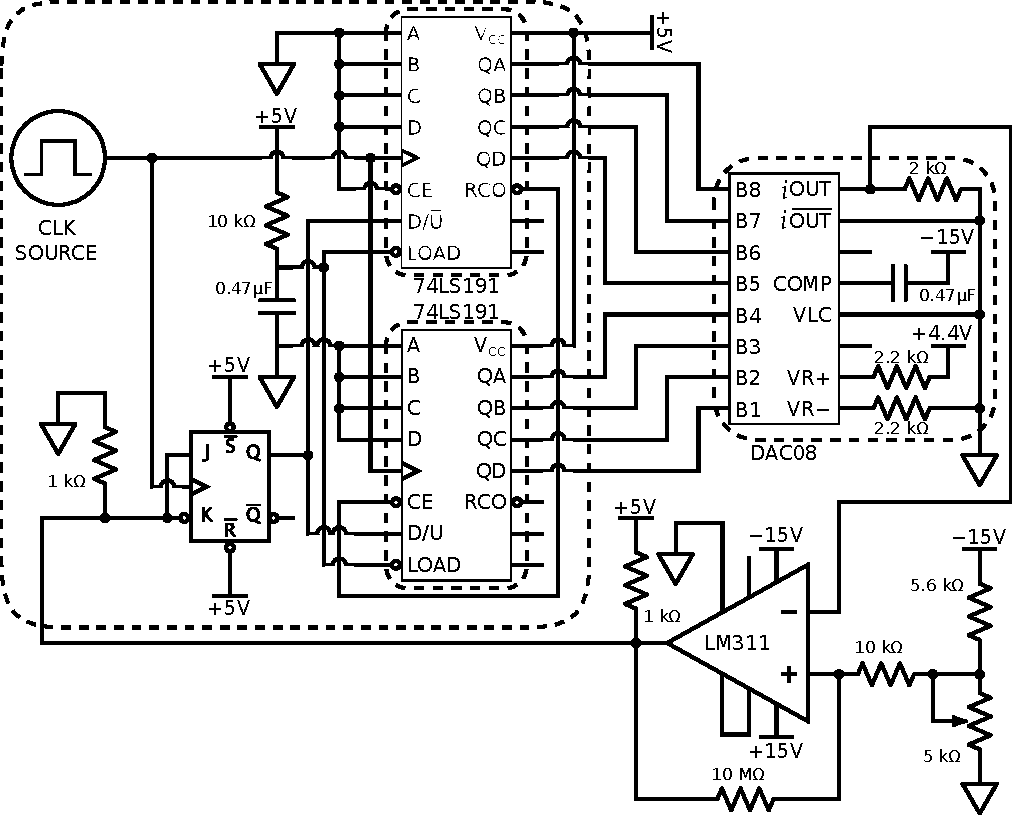
\includegraphics[width=.73\textwidth]{../E13/latex/ADC.pdf}
	\caption{}
	\label{cir13:ADC}
\end{figure}

Come vediamo, gran parte del circuito corrisponde al convertitore digitale-analogico pilotato a 8 bit già realizzato nella scorsa esperienza. In questo caso abbiamo però aggiunto un comparatore veloce con isteresi (LM311) che, come vediamo, compara il segnale in ingresso con quello del convertitore digitale-analogico. È interessante notare come l'isteresi sia stata fatta utilizzando una resistenza da \SI{10}{\kilo\ohm} e una da \SI{10}{\mega\ohm}. Così facendo abbiamo limitato l'effetto che l'uscita del LM311 ha sull'ingresso non invertente, in quanto partitore di tensione. Avendo collegato l'uscita del comparatore al JK, abbiamo un sistema automatico di controllo up/down del contatore. Il segnale in uscita dal convertitore digitale-analogico oscillerà dunque attorno al valore di tensione in ingresso. Infatti se il segnale $V_{in}$ è minore di quello in uscita dal DAC, avremo in uscita dal comparatore 0 e dunque l'ingresso J e /K del FF-JK saranno a zero logico . Il contatore sarà  dunque in modalità UP e la tensione in uscita dal DAC diminuirà. Viceversa, se il segnale del convertitore DAC è minore di quello in ingresso, in contatore sarà in modalità DOWN e avremo dunque un aumento della tensione in uscita dal DAC. 

Abbiamo notato che il segnale convertito oscillava di 4 bit. Ciò è dovuto al fatto che il controllo UP/DOWN è collegato ai due 74LS191 e dunque abbiamo un ritardo di un ciclo di clock sul cambiamento di salita/discesa.

Abbiamo infine verificato il funzionamento settando una tensione in ingresso di -0.24V. Il valore digitale letto sulla basetta al led era:

$$00001111\pm10=\frac{-4 V}{255}(15\pm2)=(-0.23\pm0.03)V$$

Come vediamo, il valore digitale è compatibile con quello analogico ottenuto misurando direttamente la tensione in ingresso. Riportiamo ora un grafico ottenuto utilizzando l'oscilloscopio. 

%\begin{figure}[htpc]
%\centering
%	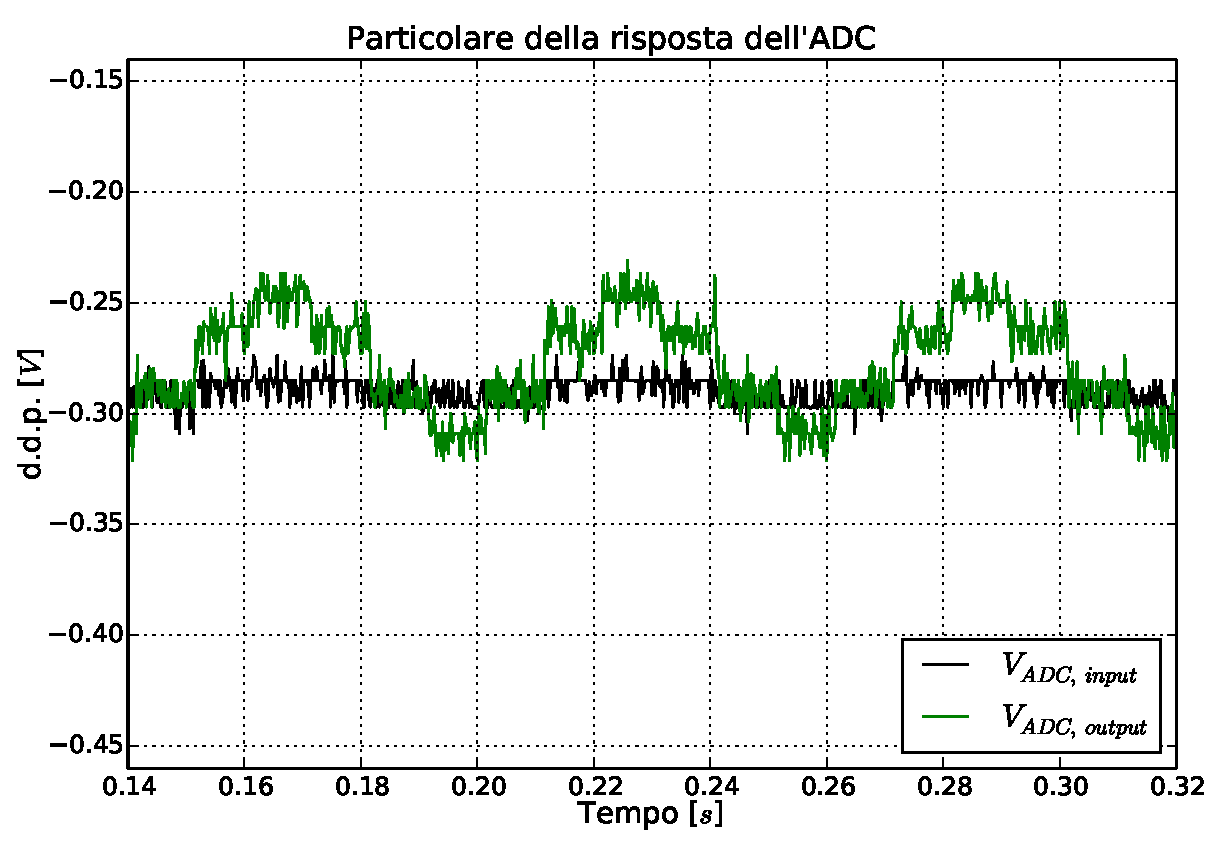
\includegraphics[width=.73\textwidth]{../E13/latex/zoom.pdf}
%	\caption{Come vediamo la presenza dell'isteresi comporta una variazione nella tensione $V_{in}$. Ciò è dovuto al fatto che la tensione è ottenuta da un partitore. Se inseriamo altri partitori, la tensione avrà dunque delle fluttuazioni. L'utilizzo della resistenza da \SI{10}{\mega\ohm} riduce drasticamente tale problema.}
%	\label{graf:zoom}
%\end{figure}

\begin{figure}[htpc]
\centering
	\begin{subfigure}[hc]{.49\textwidth}
		\centering
		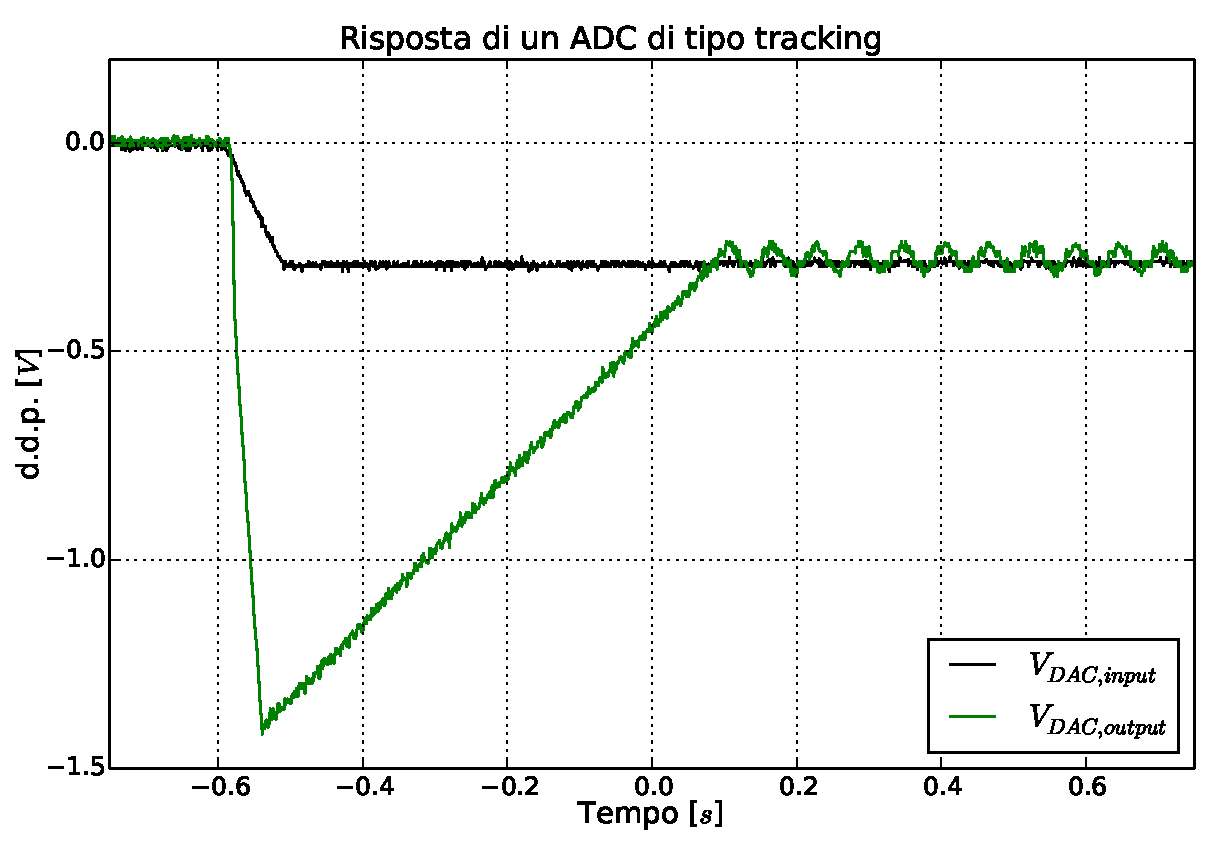
\includegraphics[width=.99\textwidth]{../E13/latex/tracker.pdf}
		\caption{}
		\label{gr13:track}
        \end{subfigure}%
        \begin{subfigure}[hc]{.49\textwidth}
		\centering
		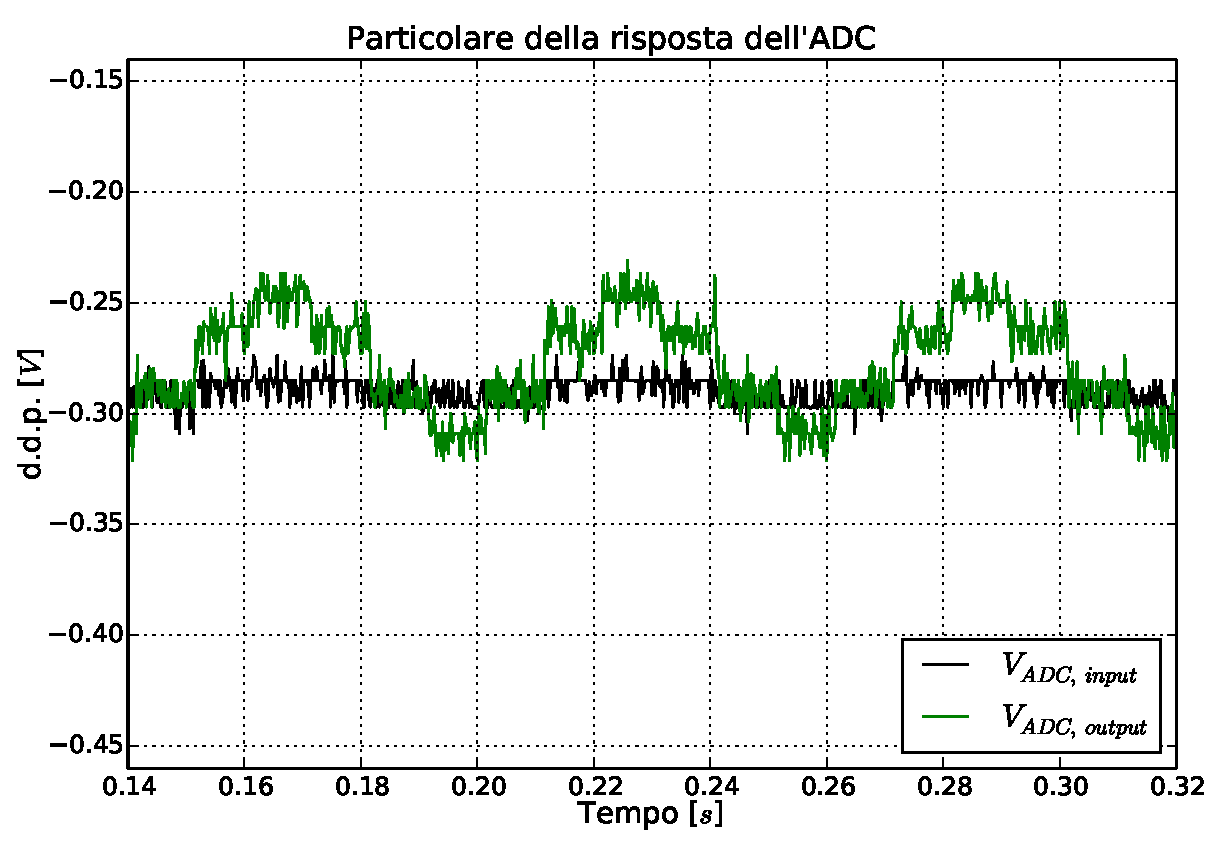
\includegraphics[width=.99\textwidth]{../E13/latex/zoom.pdf}
		\caption{}
		\label{gr13:zoom}
        \end{subfigure}
\caption{Come vediamo la tensione si stabilizza attorno al valore $V_{in}$. Come già detto, l'oscillazione di 4 bit è dovuta ai ritardi sul Clock introdotti dal controllo automatico di salita/discesa.}
\end{figure}

\subsection{Teorema del campionamento}

Il teorema del campionamento afferma che per effettuare il campionamento di un segnale senza perdita di informazione ed evitando il fenomeno dell'aliasing, la frequenza di campionamento $\nu_c$ deve essere il doppio della frequenza massima $\nu_s$ del segnale da campionare.

Bisogna però tenere presente che tale teorema è valido solo se la trasformata di Fourier del segnale da campionare è limitata nel dominio delle frequenze, cioè esiste solo una banda di frequenze in cui la trasformata non è nulla.

\subsection{Campionamento di una funzione sinusoidale}

Consideriamo una funzione $f(t)=Asin(\omega_0 t)$ e per comodità scegliamo la costante A=1. Ricordando la notazione complessa, $f(t)=\frac{e^{j\omega_0 t}-e^{-j\omega_0 t}}{2j}$, è triviale eseguire la trasformata di Fourier della funzione:

$$F(\omega)=\int_{-\infty}^{\infty} \frac{e^{j\omega_0 t}-e^{-j\omega_0 t}}{2j}e^{-j\omega t} dt=$$

Ridefiniamo $(-\omega + \omega_0)=-\omega_1$ e $(-\omega - \omega_0)=-\omega_2$. Separando ora gli integrali otteniamo:

$$F(\omega)=\int_{-\infty}^{\infty} \frac{e^{-j\omega_1 t}}{2j}dt - \int_{-\infty}^{\infty} \frac{e^{-j\omega_2 t}}{2j}dt$$

$$F(\omega)=\int_{-\infty}^{\infty} \frac{(\theta(t)+\theta(-t)) e^{-j\omega_1 t}}{2j}dt - \int_{-\infty}^{\infty} \frac{(\theta(t)+\theta(-t))e^{-j\omega_2 t}}{2j}dt$$


Introducendo un cut-off $e^{-\epsilon t}$ per gli integrali con $\theta(t)$ e $e^{\epsilon t}$ per gli integrali con $\theta(-t)$ e sfruttando le formule di Sokhotski nel liminte $\epsilon \rightarrow 0$ otteniamo:

$$F(\omega)=\pi j (\delta(\omega + \omega_0) - \delta(\omega - \omega_0))$$

Poichè noi lavoriamo con frequenze reali positive, ci interessa il modulo e solo per $\omega > 0$. Lo spettro di frequenze del seno è dunque $\pi \delta(\omega-\omega_0)$. Abbiamo una sola frequenza, come ovviamente deve essere, pari a $\frac{\omega_0}{2\pi}$. 

Le ipotesi del teorema del campionamento sono dunque verificate e possiamo studiarne le conseguenze. Per comodità definiamo $\nu_{\alpha}=\frac{\omega_{\alpha}}{2\pi}$.

%Basta usare la formula commentata sotto e si ottiene subito il risultato. Io lascio i calcoli espliciti per rompere il cazzo a chi lo corregge.

\subsubsection{$\nu_c \gg \nu_s$}

In questo caso abbiamo utilizzato $\nu_0=100 \si{\hertz}$ e $\nu_c=20 \si{\kilo\hertz}$. Siamo ampiamente entro le ipotesi del teorema e dunque la ricostruzione del segnale, come è visibile nel grafico, è molto buona. Ricordiamo che la trasformata di Fourier è eseguita sui dati utilizzando la una funzione chiamata FFT (Fast Fourier Transform). Il risultato, non avendo un set di dati continuo e infinito nel dominio non potrà ovviamente coincidere con quello ottenuto matematicamente. Tuttavia osserviamo un picco molto accentuato sulla frequenza $\nu_0$. Ciò ovviamente è corretto in quanto stiamo analizzando un funzione sinusoidale.

\begin{figure}[H]
\centering
	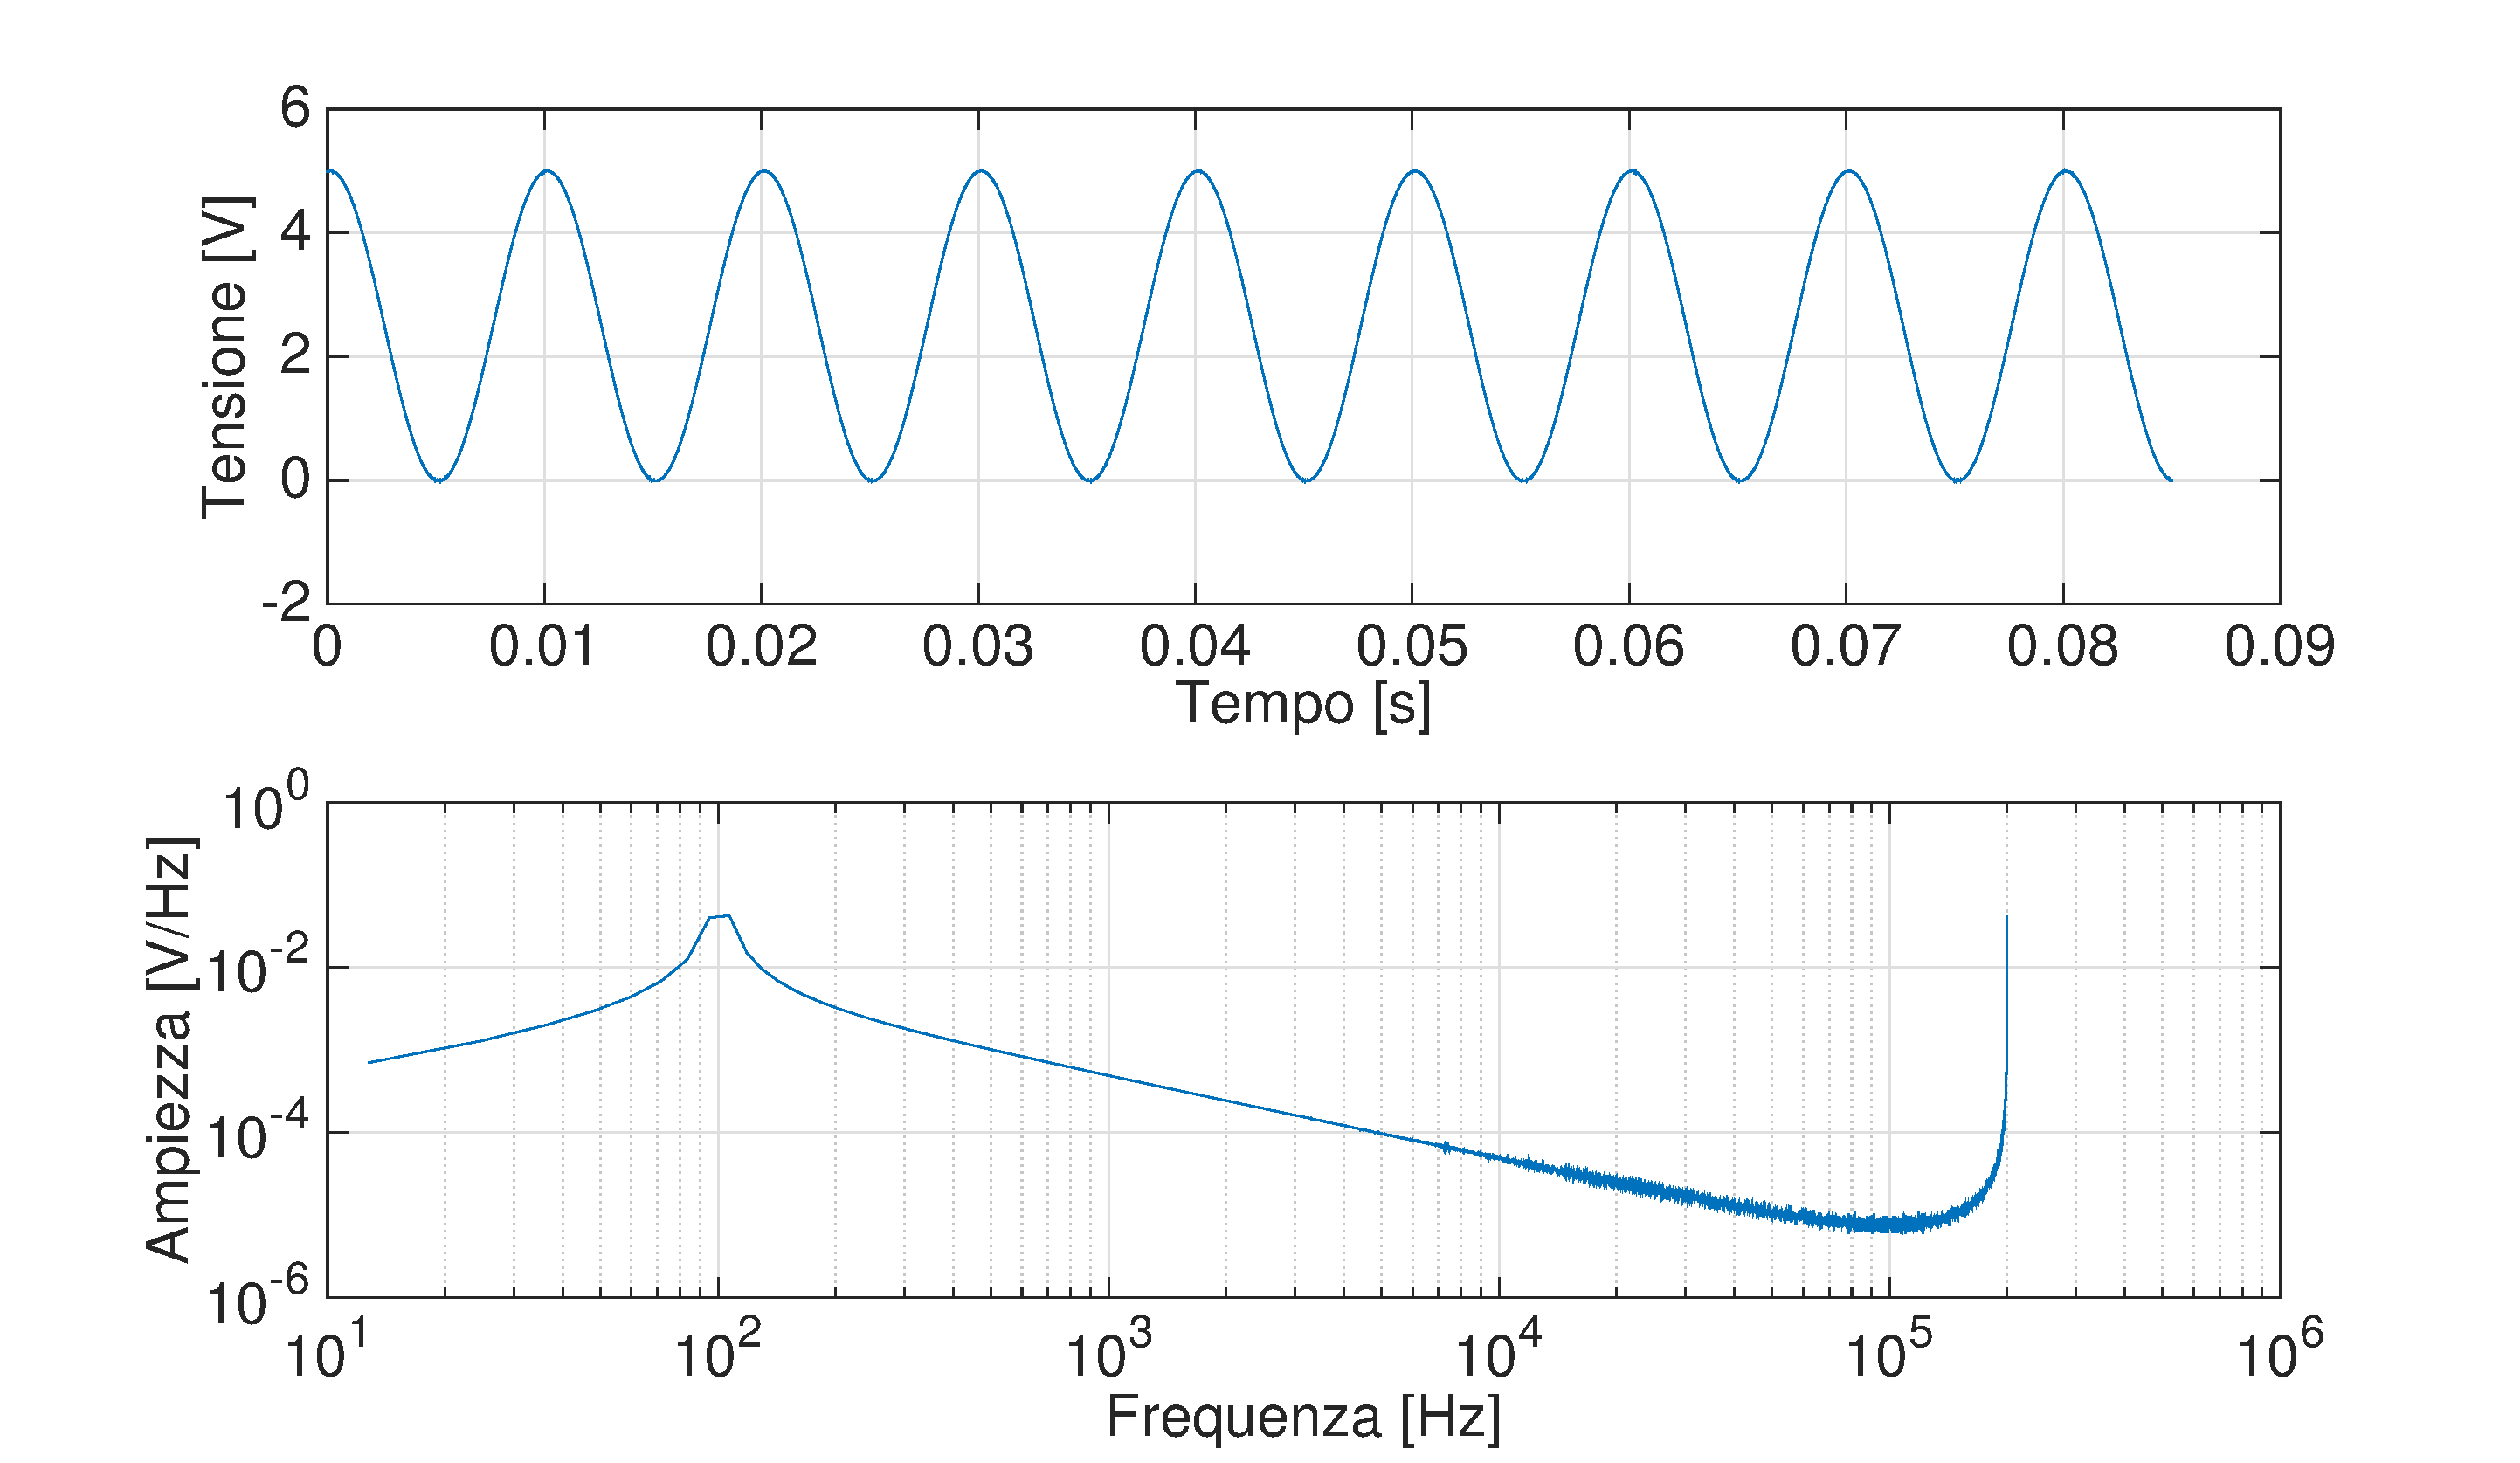
\includegraphics[width=.73\textwidth]{../E13/latex/sin100hz@17000,200000.pdf}
	\caption{Come vediamo dal grafico, abbiamo una frequenza principale a $\nu_0=100 \si{\hertz}$. Il picco dopo i $10^5\si{\hertz}$ è dovuto all'algoritmo della FFT.}
	\label{sin1}
\end{figure}





%\subsubsection{ $f_s<f_c<2f_s$}


%In questo caso abbiamo utilizzato una $\nu_0=100 \si{\hertz}$ e $\nu_c=$. Ci troviamo in una situazione in cui il segnale si riesce ancora a ricostruire ma risulta distorto. Anche la trasformata di Fourier è molto distorta. Un campionamento così fatto fa perdere informazioni al segnale con la conseguenza che non potrà essere ricostruito correttamente.


\subsubsection{ $\nu_c = \nu_s$}

In questo caso abbiamo utilizzato $\nu_0=\nu_c=100 \si{\hertz}$. Il segnale risulta irriconoscibile e non si può sapere quale segnale sia stato campionato. Nemmeno la FFT porta informazioni in quanto abbiamo picchi distribuiti senza alcuna correlazione. Non si riesce dunque a ricavare nessuna informazione dal campionamento

\begin{figure}[H]
\centering
	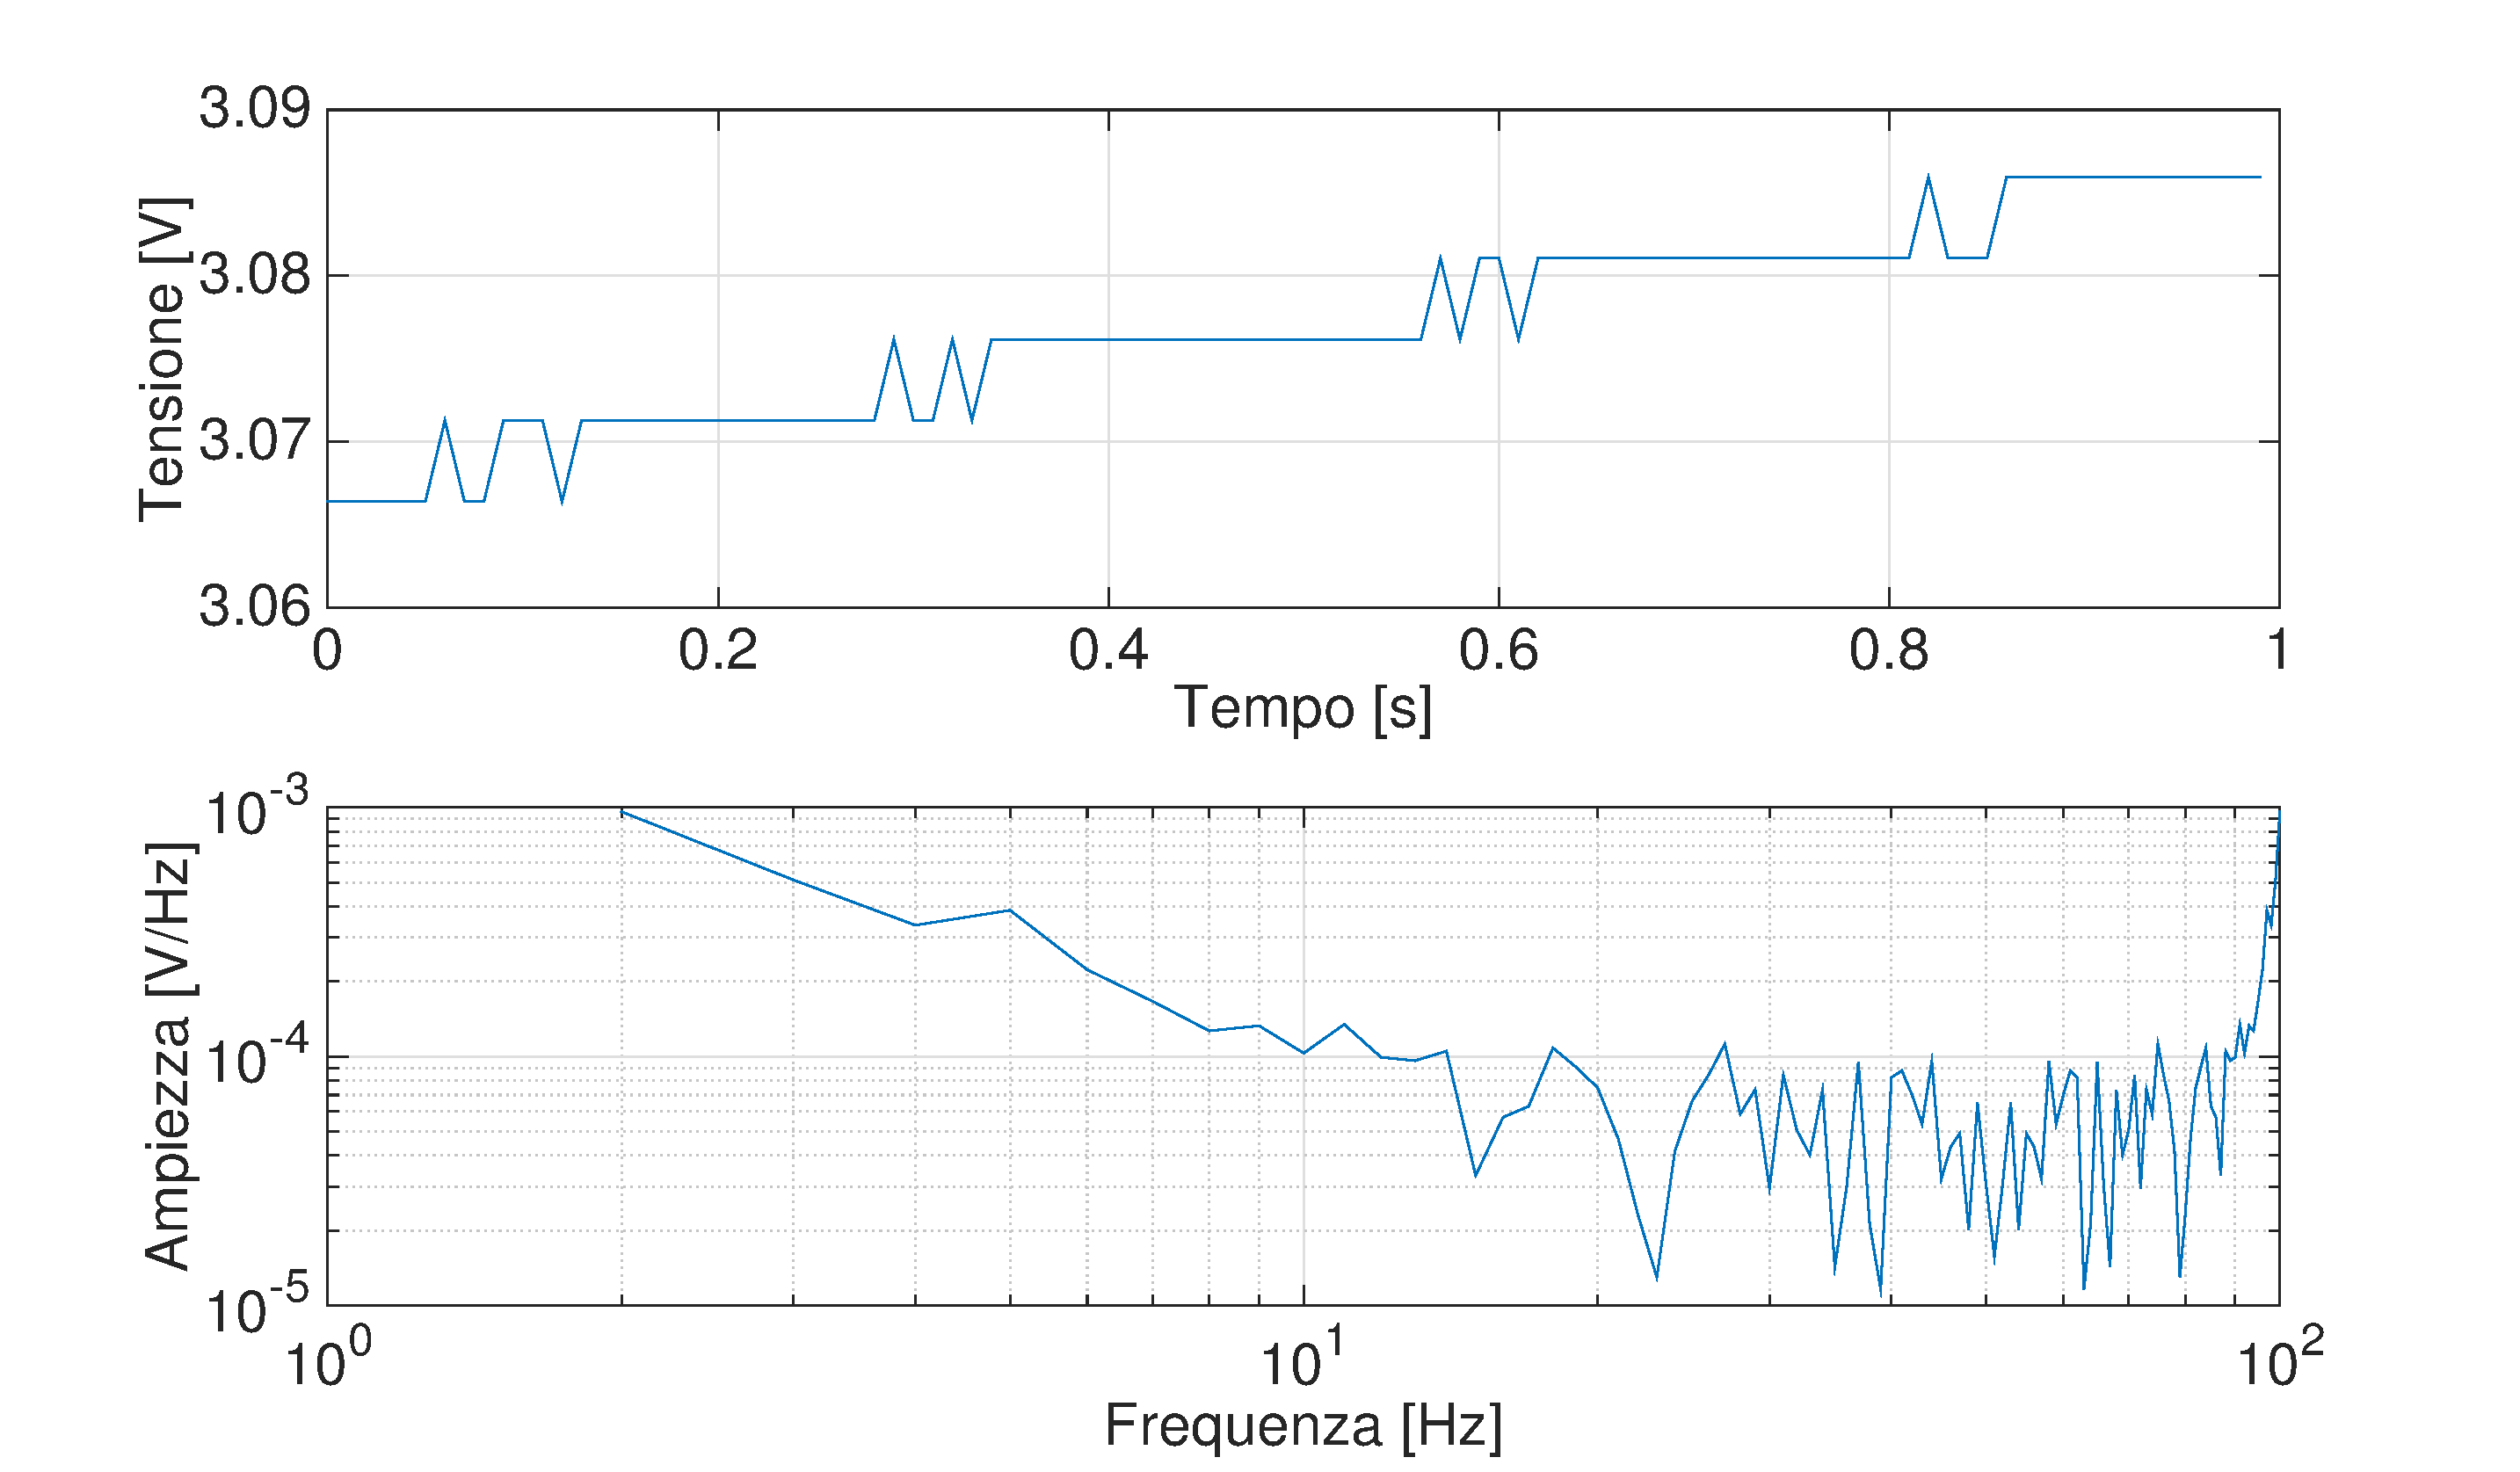
\includegraphics[width=.73\textwidth]{../E13/latex/sin100hz@100,100_2.pdf}
	\caption{Come già accennato i dati raccolti utilizzando una frequenza di campionamento uguale a quella del segnale in ingresso non permettono una ricostruzione corretta del segnale. }
	\label{sin2}
\end{figure}

\subsubsection{ $\nu_c \approx \nu_s$}
In questo caso abbiamo utilizzato $\nu_0=100 \si{\hertz}$ e $\nu_c=97 \si{\hertz}$. Notiamo che avendo utilizzato una frequenza di campionamento più bassa, otteniamo un forma d'onda che in realtà non esiste. Il campionamento fatto con queste frequenze infatti perde più di un periodo della sinusoidale ad ogni punto, e dunque otteniamo una forma d'onda che non porta informazioni rispetto a quella in ingresso.

\begin{figure}[H]
\centering
	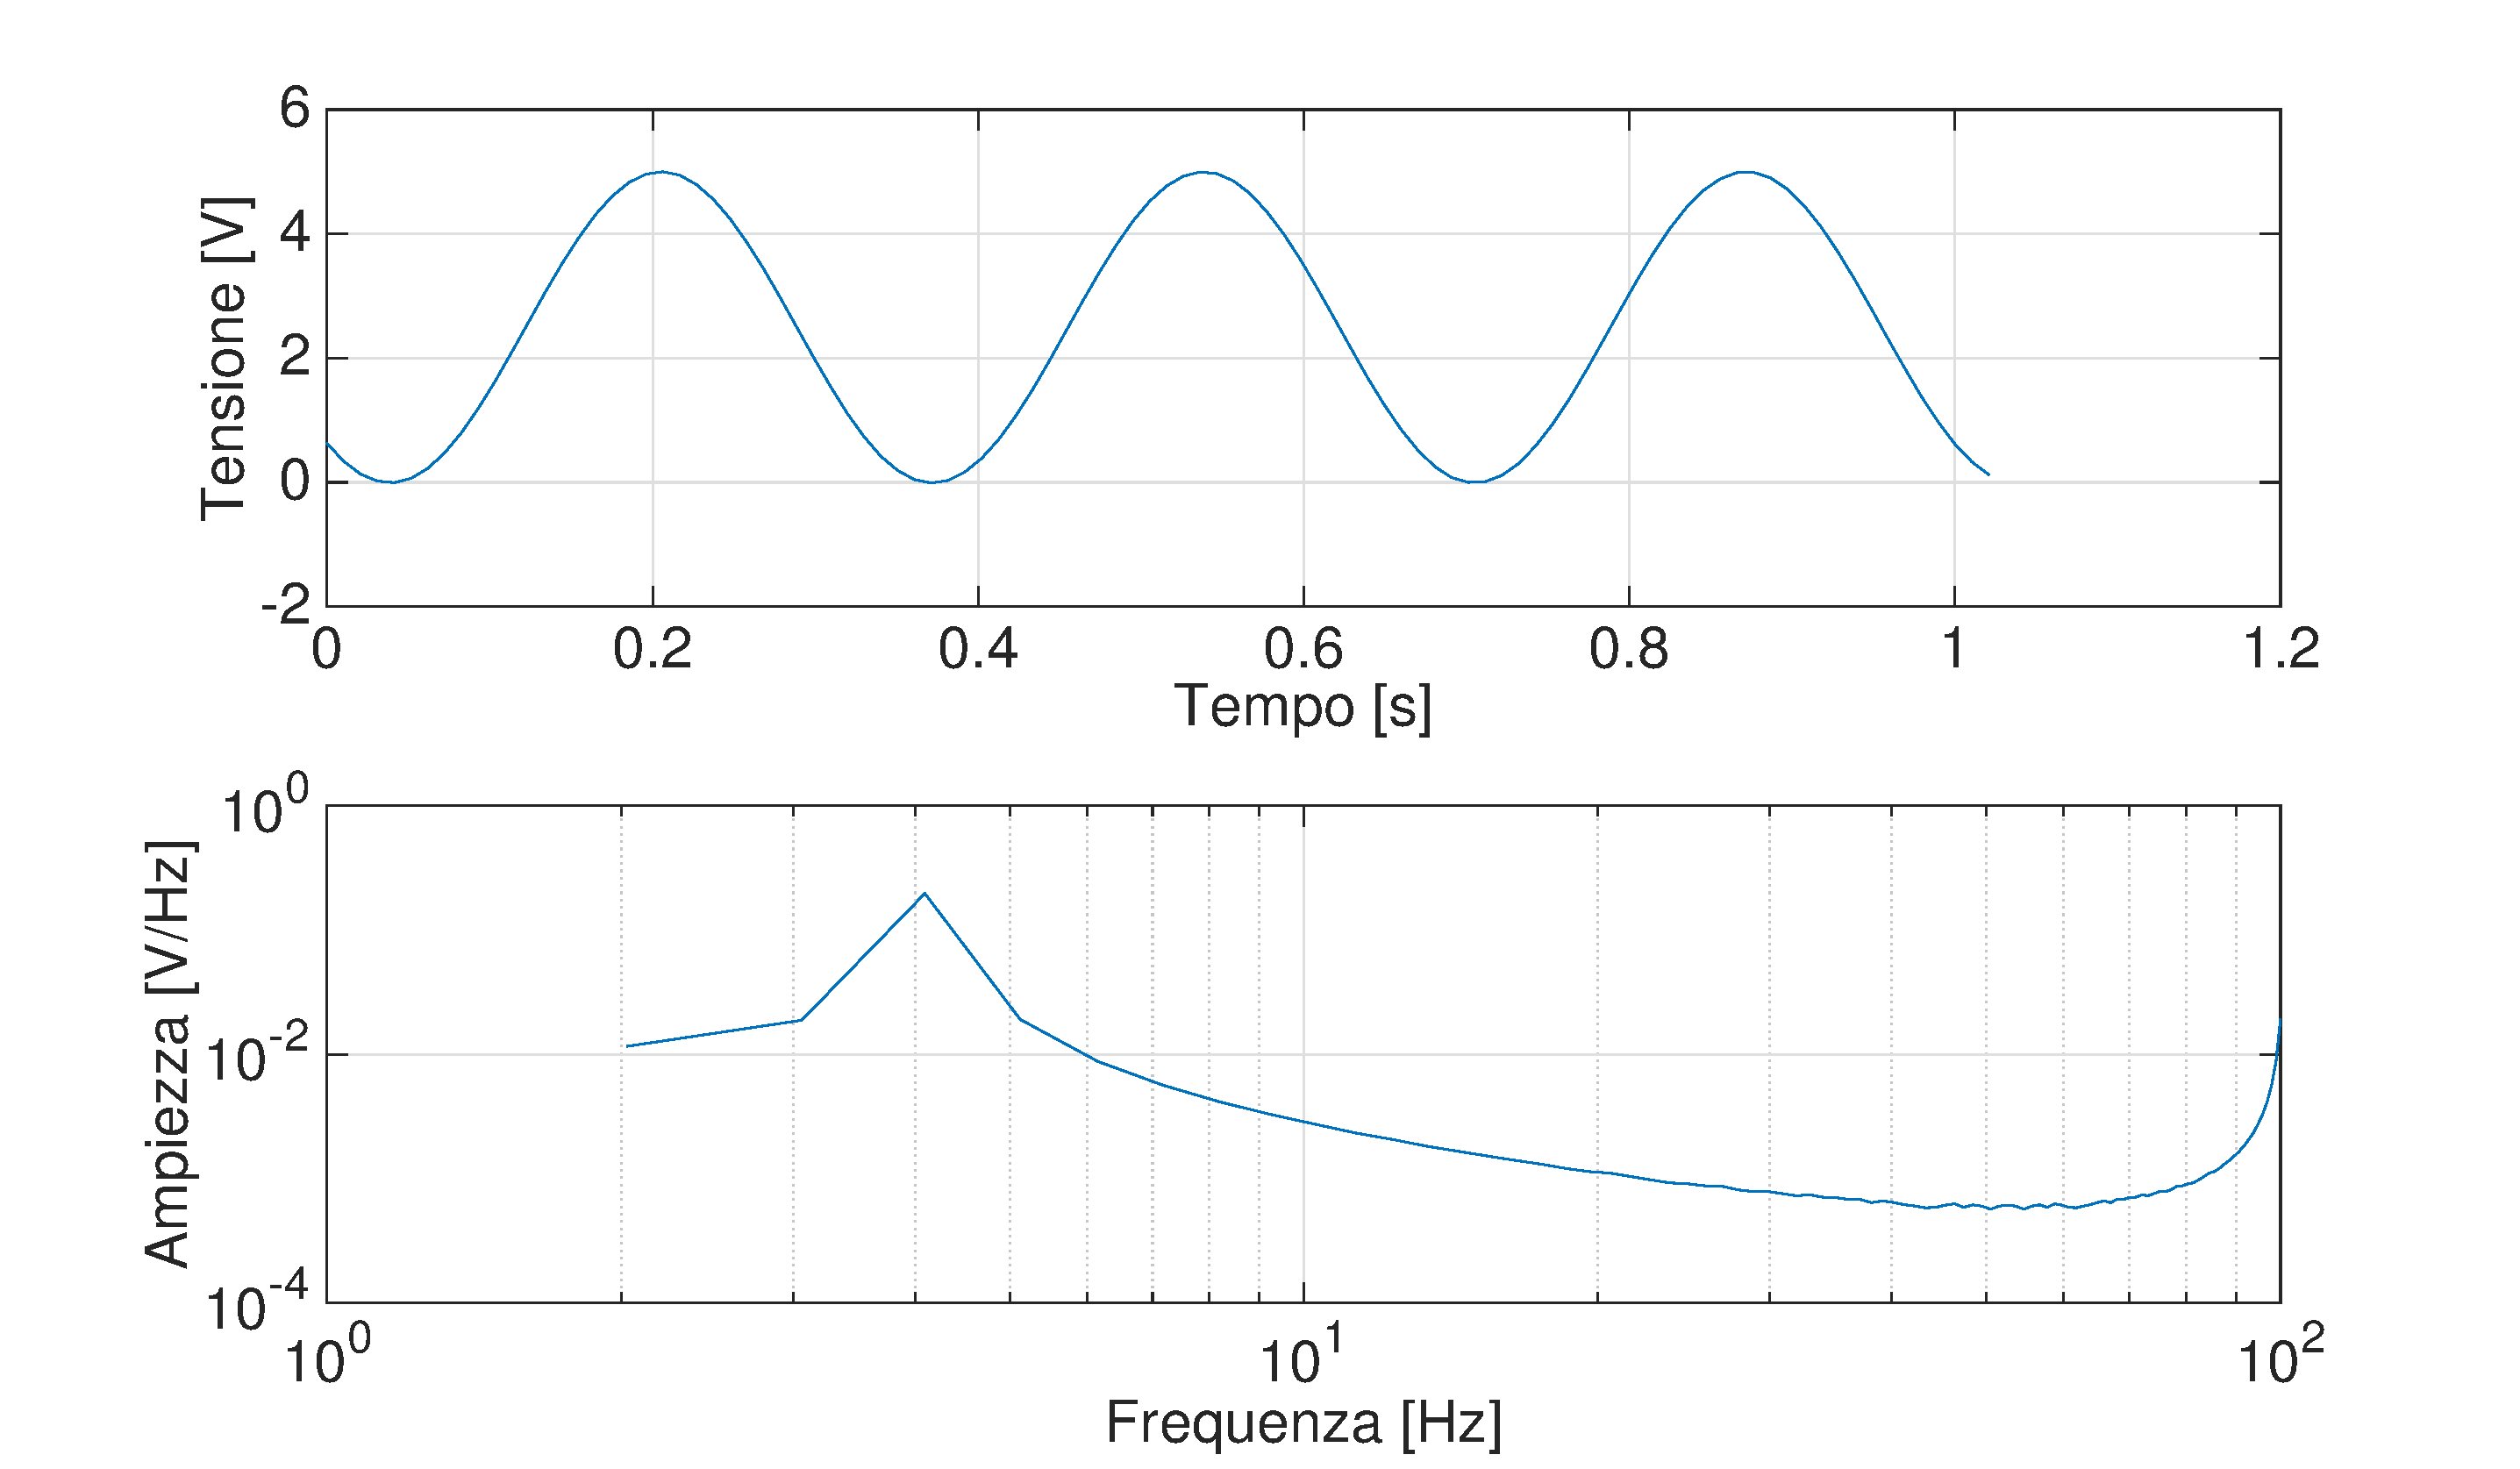
\includegraphics[width=.73\textwidth]{../E13/latex/sin100hz@100,97.pdf}
	\caption{Come vediamo dal grafico, la forma d'onda campionata è una sinusoide con una frequenza di alcuni Hz. Ciò è dovuto al fatto che la frequenza di campionamento è leggermente inferiore alla frequenza del segnale in ingresso e dunque abbiamo un piccolo ritardo che si propaga a cascata su ogni dati successivo. Il risultato è una forma d'onda con una frequenza circa uguale alla differenza tra $\nu_0$ e $\nu_c$.}
	\label{sin3}
\end{figure}



\subsection{Campionamento di altre forme d'onda}
Abbiamo campionato altre forme d'onda, ricordando l'importante condizione $\nu_c>2\nu_s$. Nella ricostruzione delle forme d'onda con serie di Fourier è stata ovviamente trascurata una costante A che può essere aggiunta alla fine per linearità. Ciò non è essenziale comunque per le osservazione che faremo noi.


\subsubsection{onda quadra}
Abbiamo utilizzato un'onda quadra di frequenza $\nu_0=100 \si{\hertz}$ e una frequenza di campionamento di $\nu_c=20\si{\kilo\hertz}$. Come vediamo, la forma d'onda è stata campionata senza distorsioni sebbene il teorema del campionamento non sia valido. Infatti lo spettro di frequenze non è limitato, come mostreremo in seguito.

Essendo un'onda periodica possiamo calcolarne direttamente la serie di Fourier. Osserviamo anzitutto che la funzione è dispari se consideriamo l'onda quadra come: 

\begin{displaymath}
f(t):=
\begin{cases}
-1 \quad se \quad -\frac{\tau}{2}<t<0 \\
+1 \quad se \quad 0<t<\frac{\tau}{2} \\ 
\end{cases}
\end{displaymath}

Lo sviluppo in serie di Fourier risulta dunque: 

\begin{equation}
f(t)=\sum_{n=0}^{+\infty}\frac{4}{(2n+1)\pi}sin (\frac{2\pi(2n+1)}{\tau}t)
\end{equation}

Vediamo immediatamente come nella serie compaiano solo le armoniche dispari, ovvero $\nu_n=\frac{2n+1}{\tau}=(2n+1)\nu_0$. Ciò è effettivamente verificato dalla FFT dei dati da noi campionati.

Notiamo che $n$ è definito da 0 ad infinito. Dunque lo spettro delle frequenze non è limitato. Dunque non vale il teorema del campionamento. Tuttavia, essendo i coefficienti di fourier proporzionali a $\frac{1}{n}$, è evidente che le armoniche con frequenze alte avranno un impatto sulla ricostruzione del segnale minore che le prime armoniche. È dunque sufficiente, per ottenere un buon campionamento, utilizzare una frequenza di qualche fattore maggiore rispetto alle prime armoniche. 

%Per completezza ricordiamo che è possibile anche ottenere lo spettro della $f(t)$ utilizzando direttamete le trasformate di Fourier. È infatti sufficiente ricordare che la trasformata di Fourier di una funzione periodica con periodo $2\pi$ è semplicemente:

%$$F(f(t))(\omega)=2\pi \sum_{n=-\infty}^{+\infty} c_n \delta(\omega-n ) $$

%dove i coefficienti $c_n=\frac{1}{2\pi}\int_{-\pi}^{+\pi} f(t)e^{-int}dt$.

%Il risultato è lo stesso di quello sopra calcolato. Notiamo inoltre che le $\nu_n$ sono quantizzate.

\begin{figure}[H]
\centering
	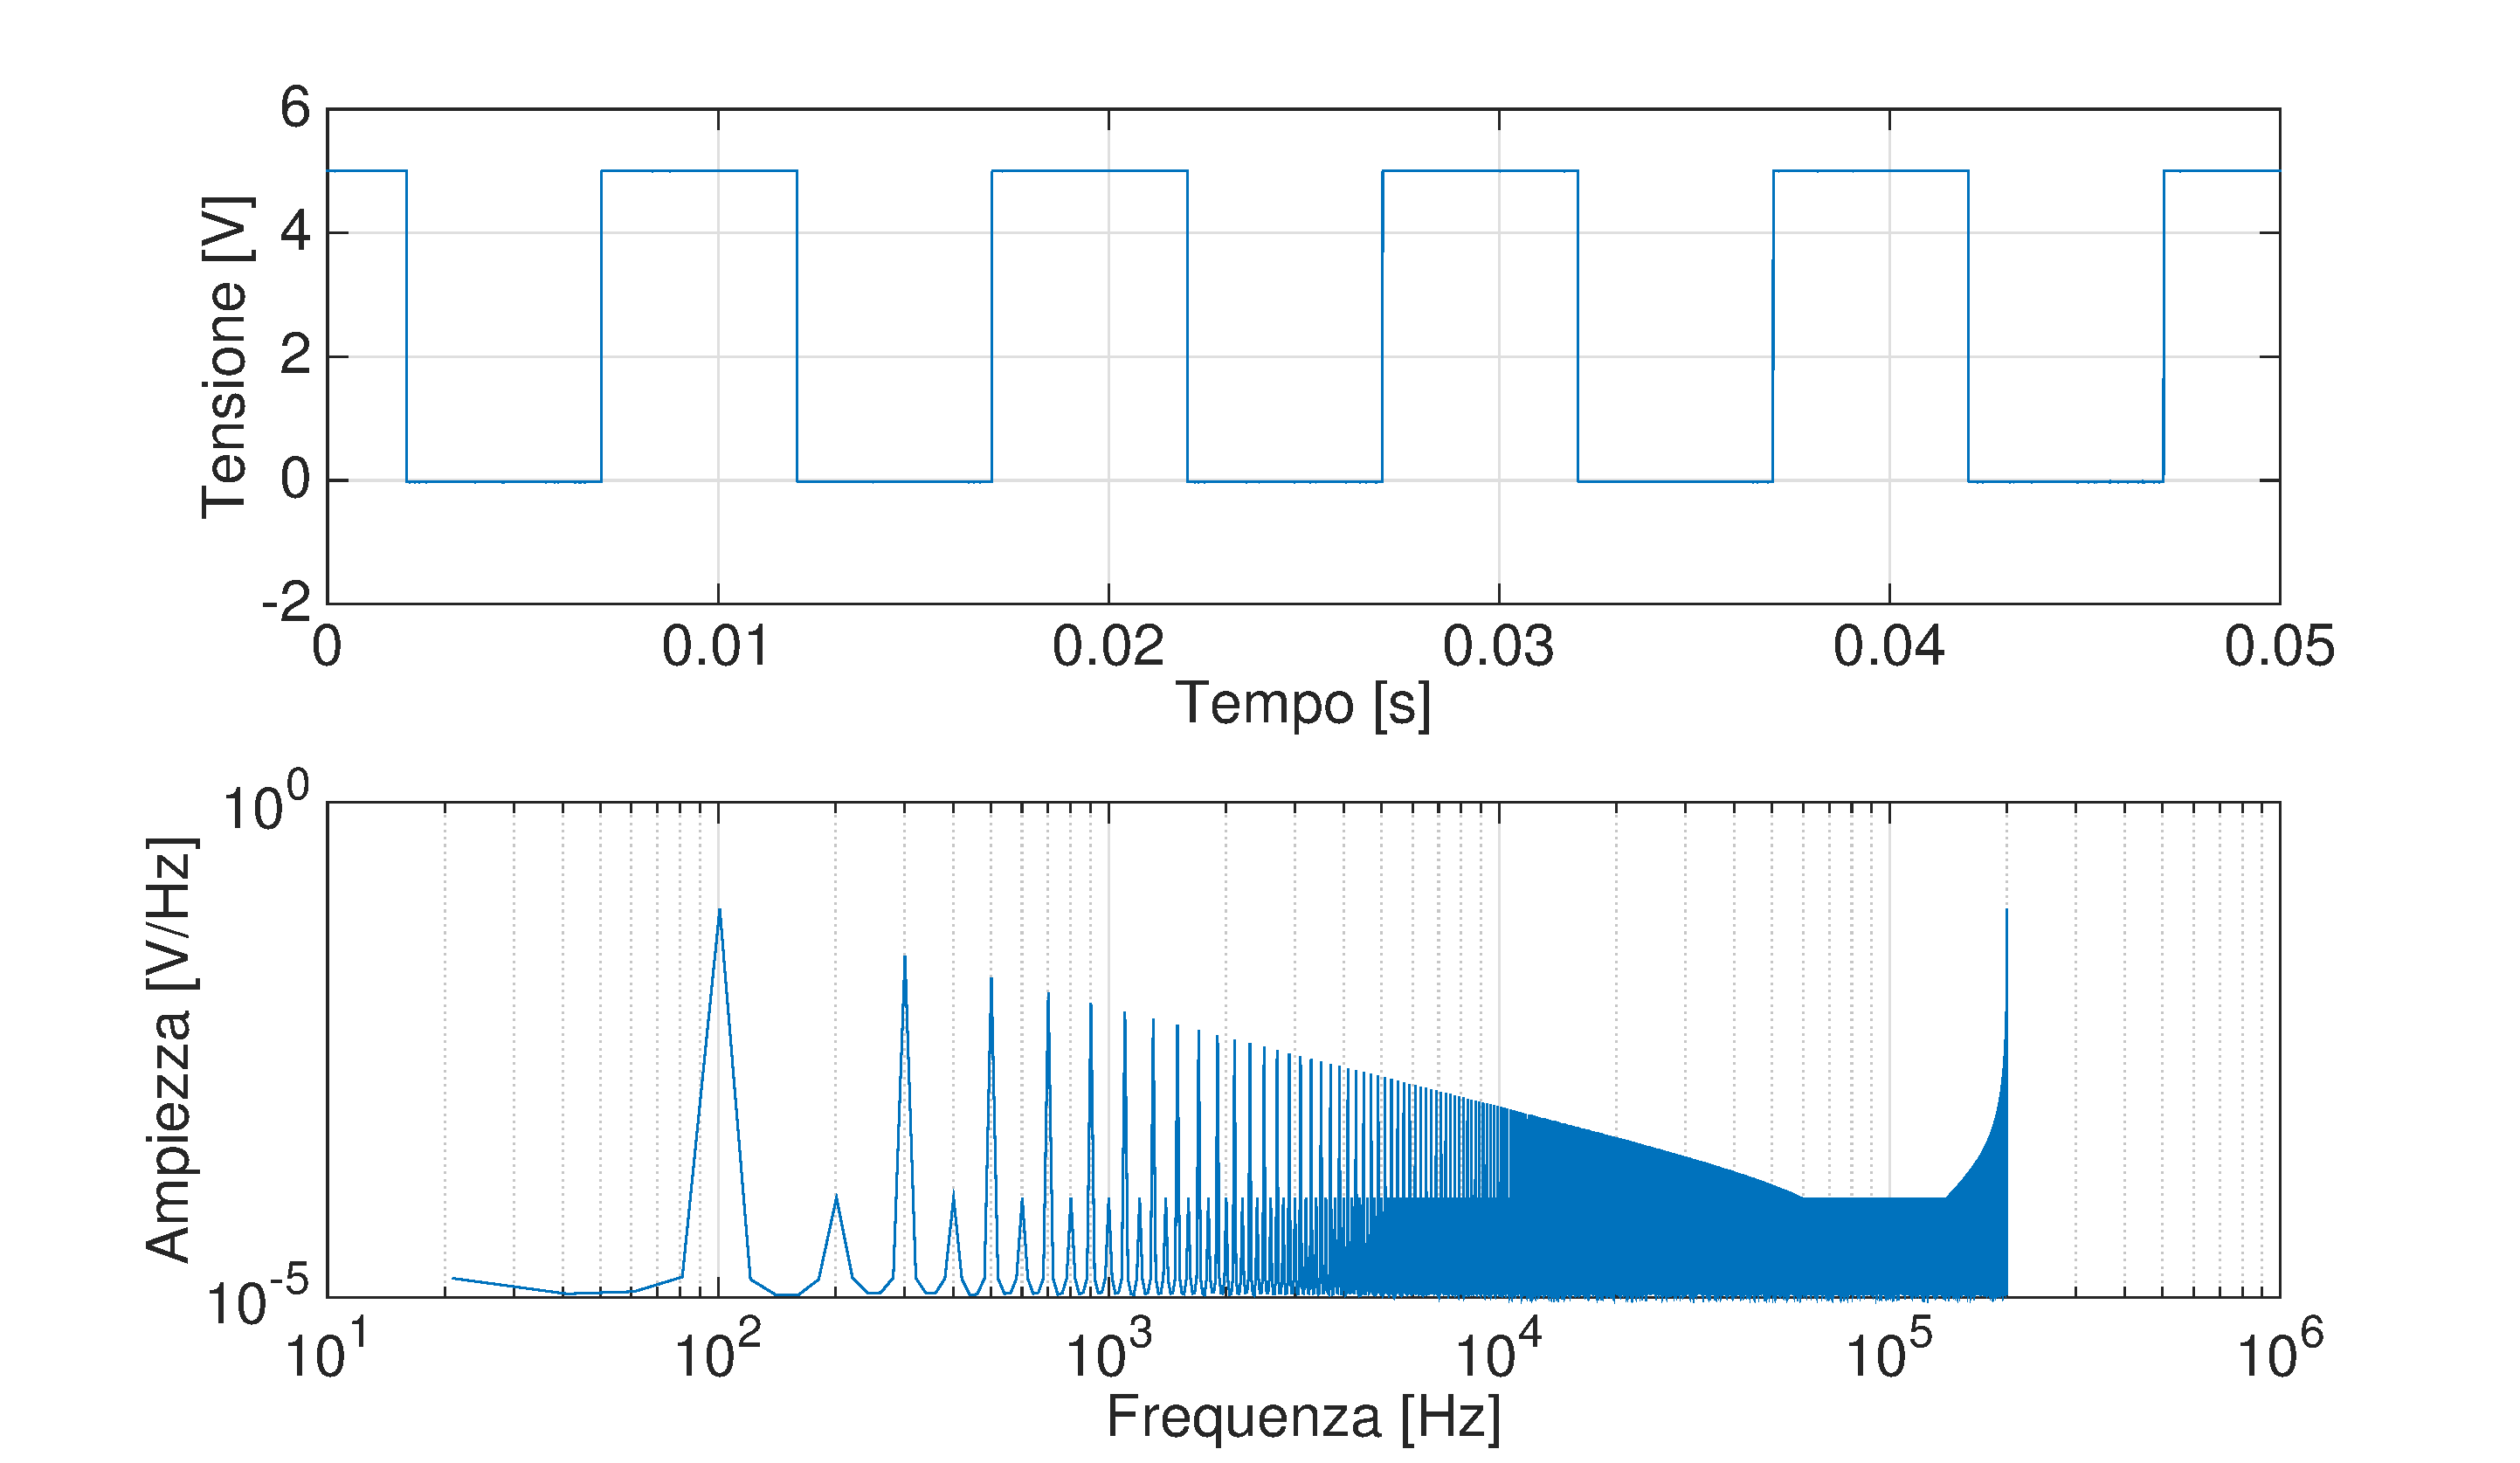
\includegraphics[width=.73\textwidth]{../E13/latex/quadra100hz@10000,200000.pdf}
	\caption{Osserviamo dal grafico che i picchi di frequenze principali sono si trovano sui multipli dispari della frequenza principale. Abbiamo tuttavia dei picchi meno accentuati anche sulle armoniche pari. Ciò è probabilmente dovuto alla limitatezza dei dati da noi raccolti.}
	\label{quadra}
\end{figure}


\subsubsection{onda triangolare}
Abbiamo utilizzato un'onda triangolare di frequenza $\nu_0=100 \si{\hertz}$ e una frequenza di campionamento di $\nu_c=20\si{\kilo\hertz}$. Come vediamo, la forma d'onda è stata anche in questo caso campionata senza distorsioni. La funzione può essere scritta sfruttando la simmetria come:

\begin{displaymath}
f(t):=
\begin{cases}
1+\frac{4}{\tau}t \quad se \quad -\frac{\tau}{2}<t<0 \\
1-\frac{4}{\tau}t \quad se \quad 0<t<\frac{\tau}{2} \\ 
\end{cases}
\end{displaymath}

Lo sviluppo in serie di Fourier di tale funzione è:

\begin{equation}
f(t)=\sum_{n=0}^{+\infty}\frac{8}{(2n+1)^2\pi^2}cos (\frac{2\pi(2n+1)}{\tau}t)
\end{equation}

Come vediamo anche in questo caso abbiamo solo le armoniche dispari, ovvero $\nu_n=\frac{2n+1}{\tau}=(2n+1)\nu_0$. Osservando la FFT dei dati vediamo che ciò è corretto. 

\begin{figure}[H]
\centering
	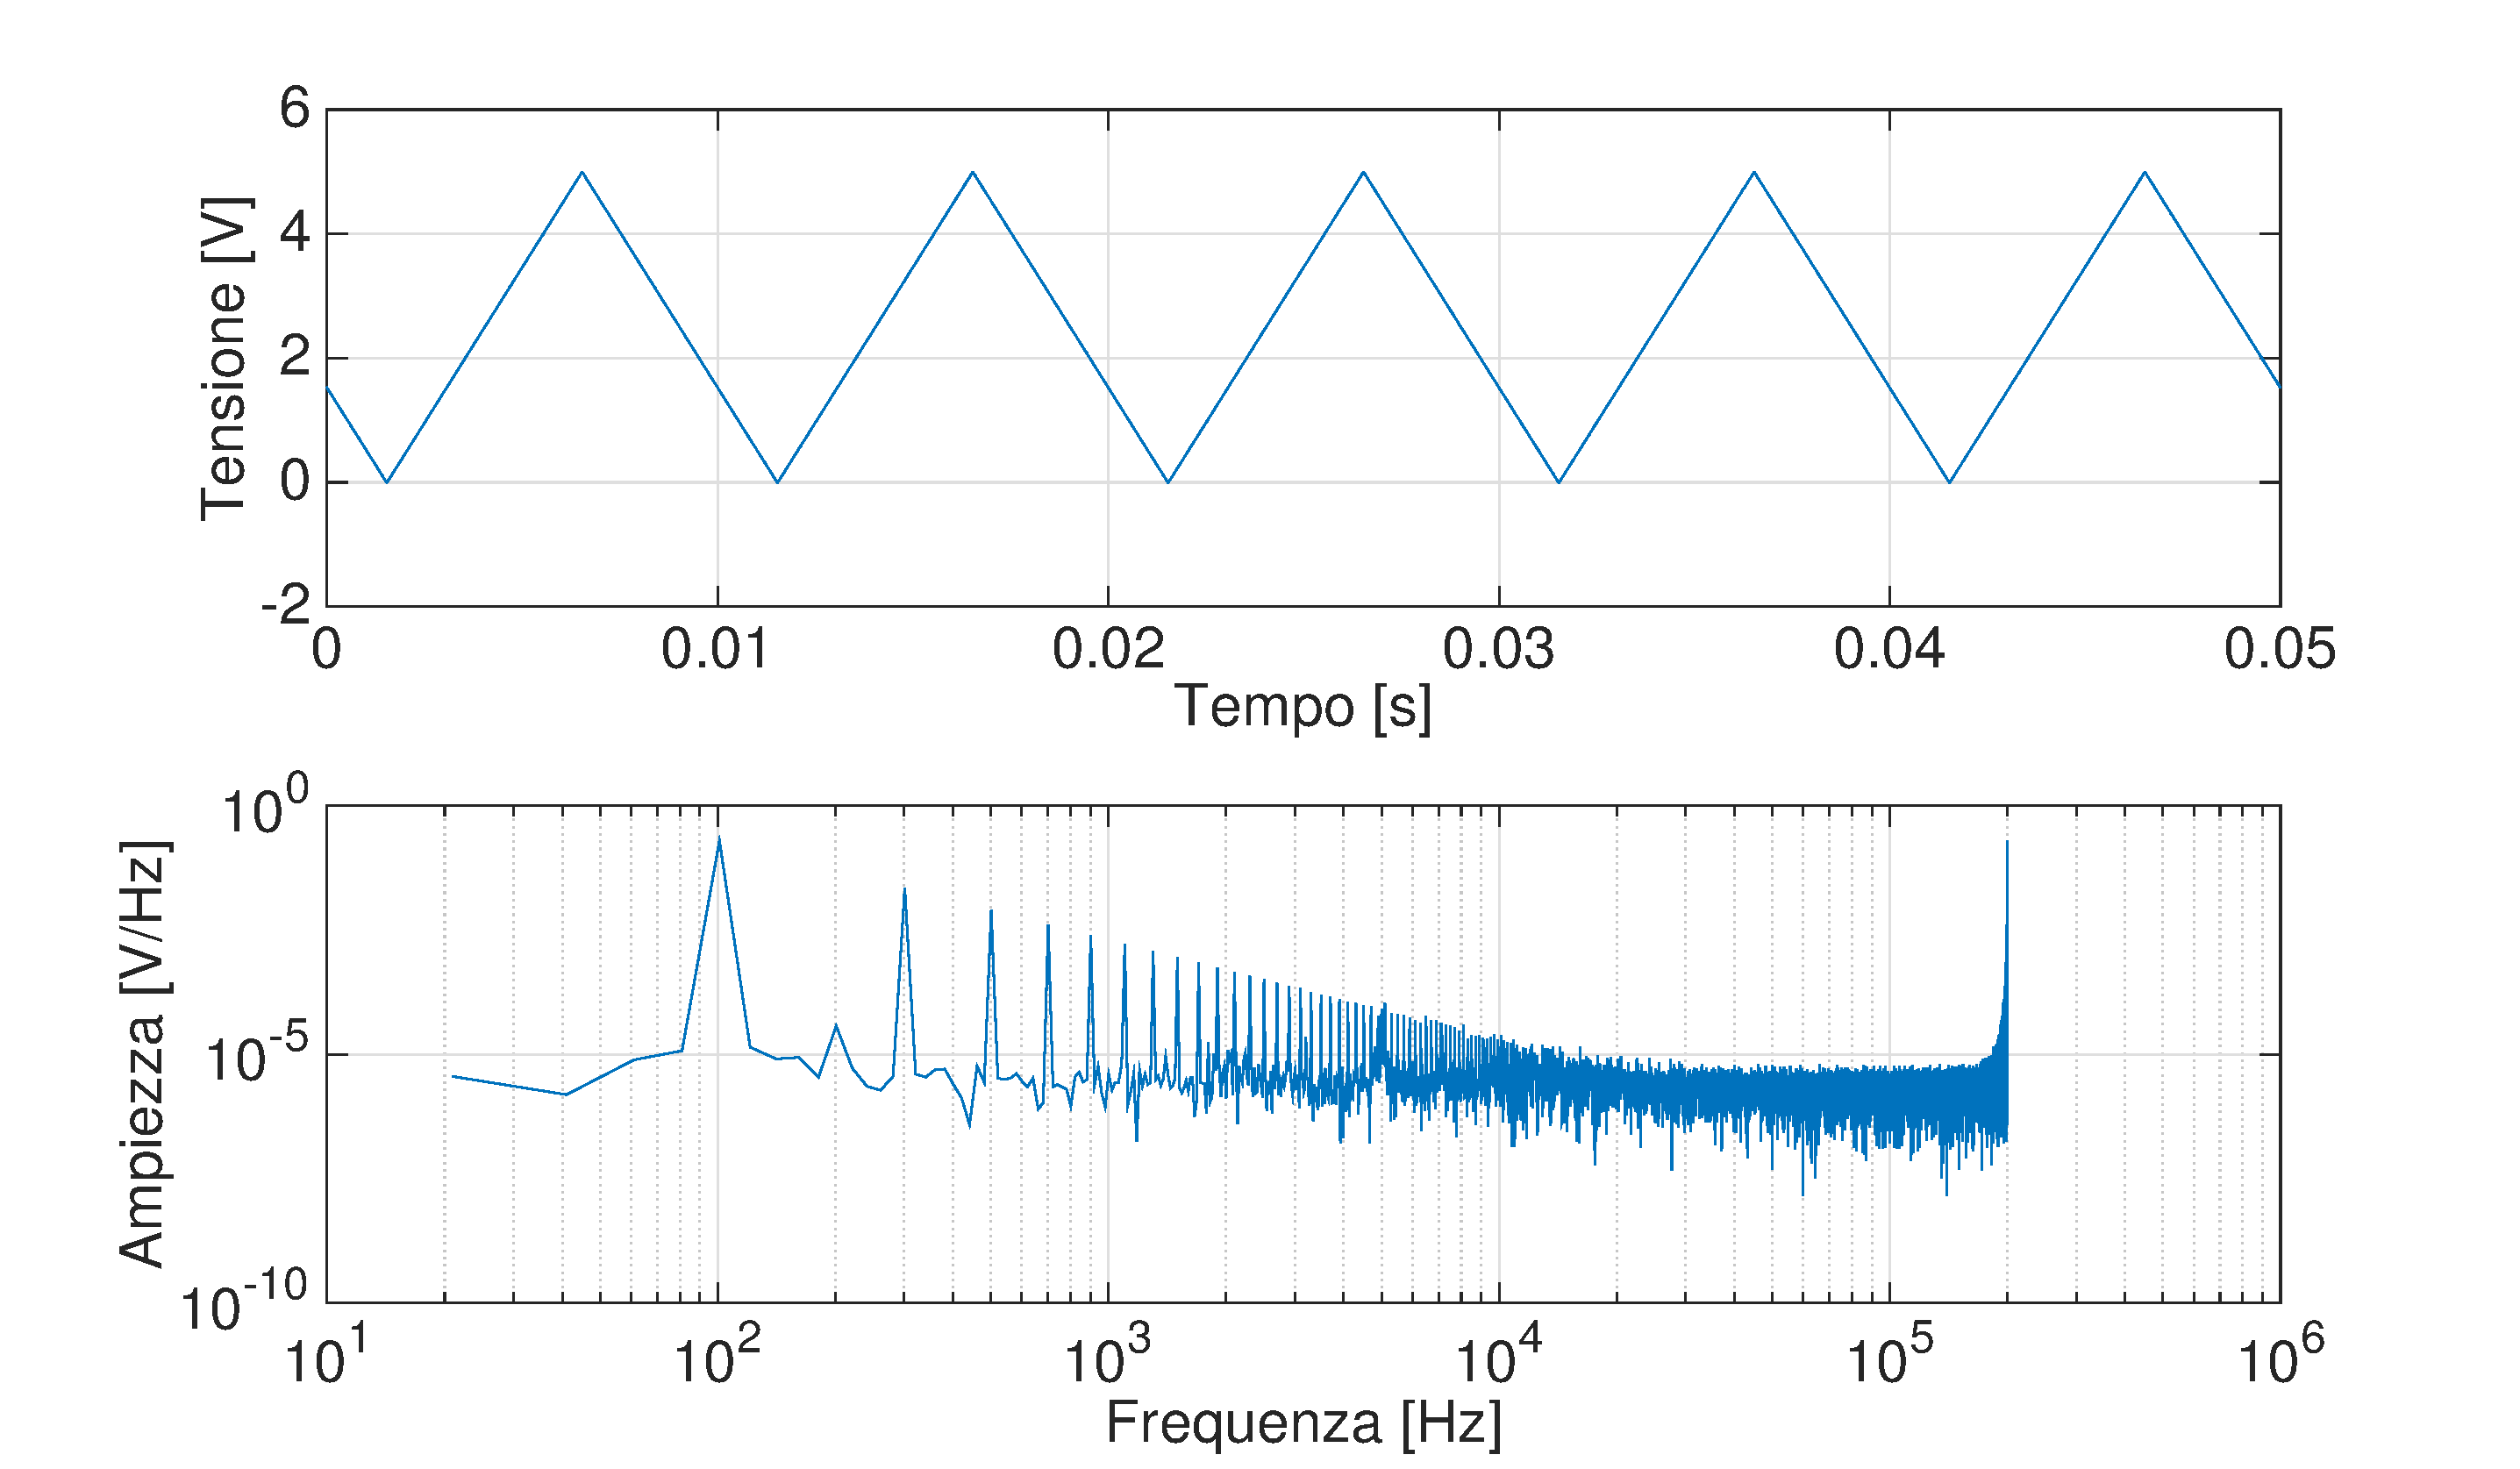
\includegraphics[width=.73\textwidth]{../E13/latex/triangolare100hz@10000,200000.pdf}
	\caption{Anche in questo caso sono ben visibili i picchi di frequenza sulle armoniche dispari. }
	\label{triangolare}
\end{figure}

\subsubsection{onda dente di sega}

Abbiamo utilizzato un'onda a dente di sega di frequenza $\nu_0=100 \si{\hertz}$ e una frequenza di campionamento di $\nu_c=20\si{\kilo\hertz}$. Sebbene non valga il teorema del campionamento abbiamo ottenuto un segnale non distorto. Ciò è dovuto, come ai casi sopra, alla preponderanza delle prime armoniche.

Scriviamo l'onda a dente di sega come: 

$$f(t):= \frac{2}{\tau}t \quad -\frac{\tau}{2}<t<\frac{\tau}{2}$$

Lo sviluppo in serie di Fourier è dunque:

\begin{equation}
f(t)=2\sum_{n=1}^{+\infty}\frac{(-1)^{n-1}}{n\pi}sin (\frac{2\pi n}{\tau}t)
\end{equation}


In questo caso abbiamo sia armoniche pari che dispari. Infatti $\nu_n=\frac{n}{\tau}=n\nu_0$. Anche in questo caso ciò è confermato dai dati sperimentali riguardanti la FFT. 

\begin{figure}[H]
\centering
	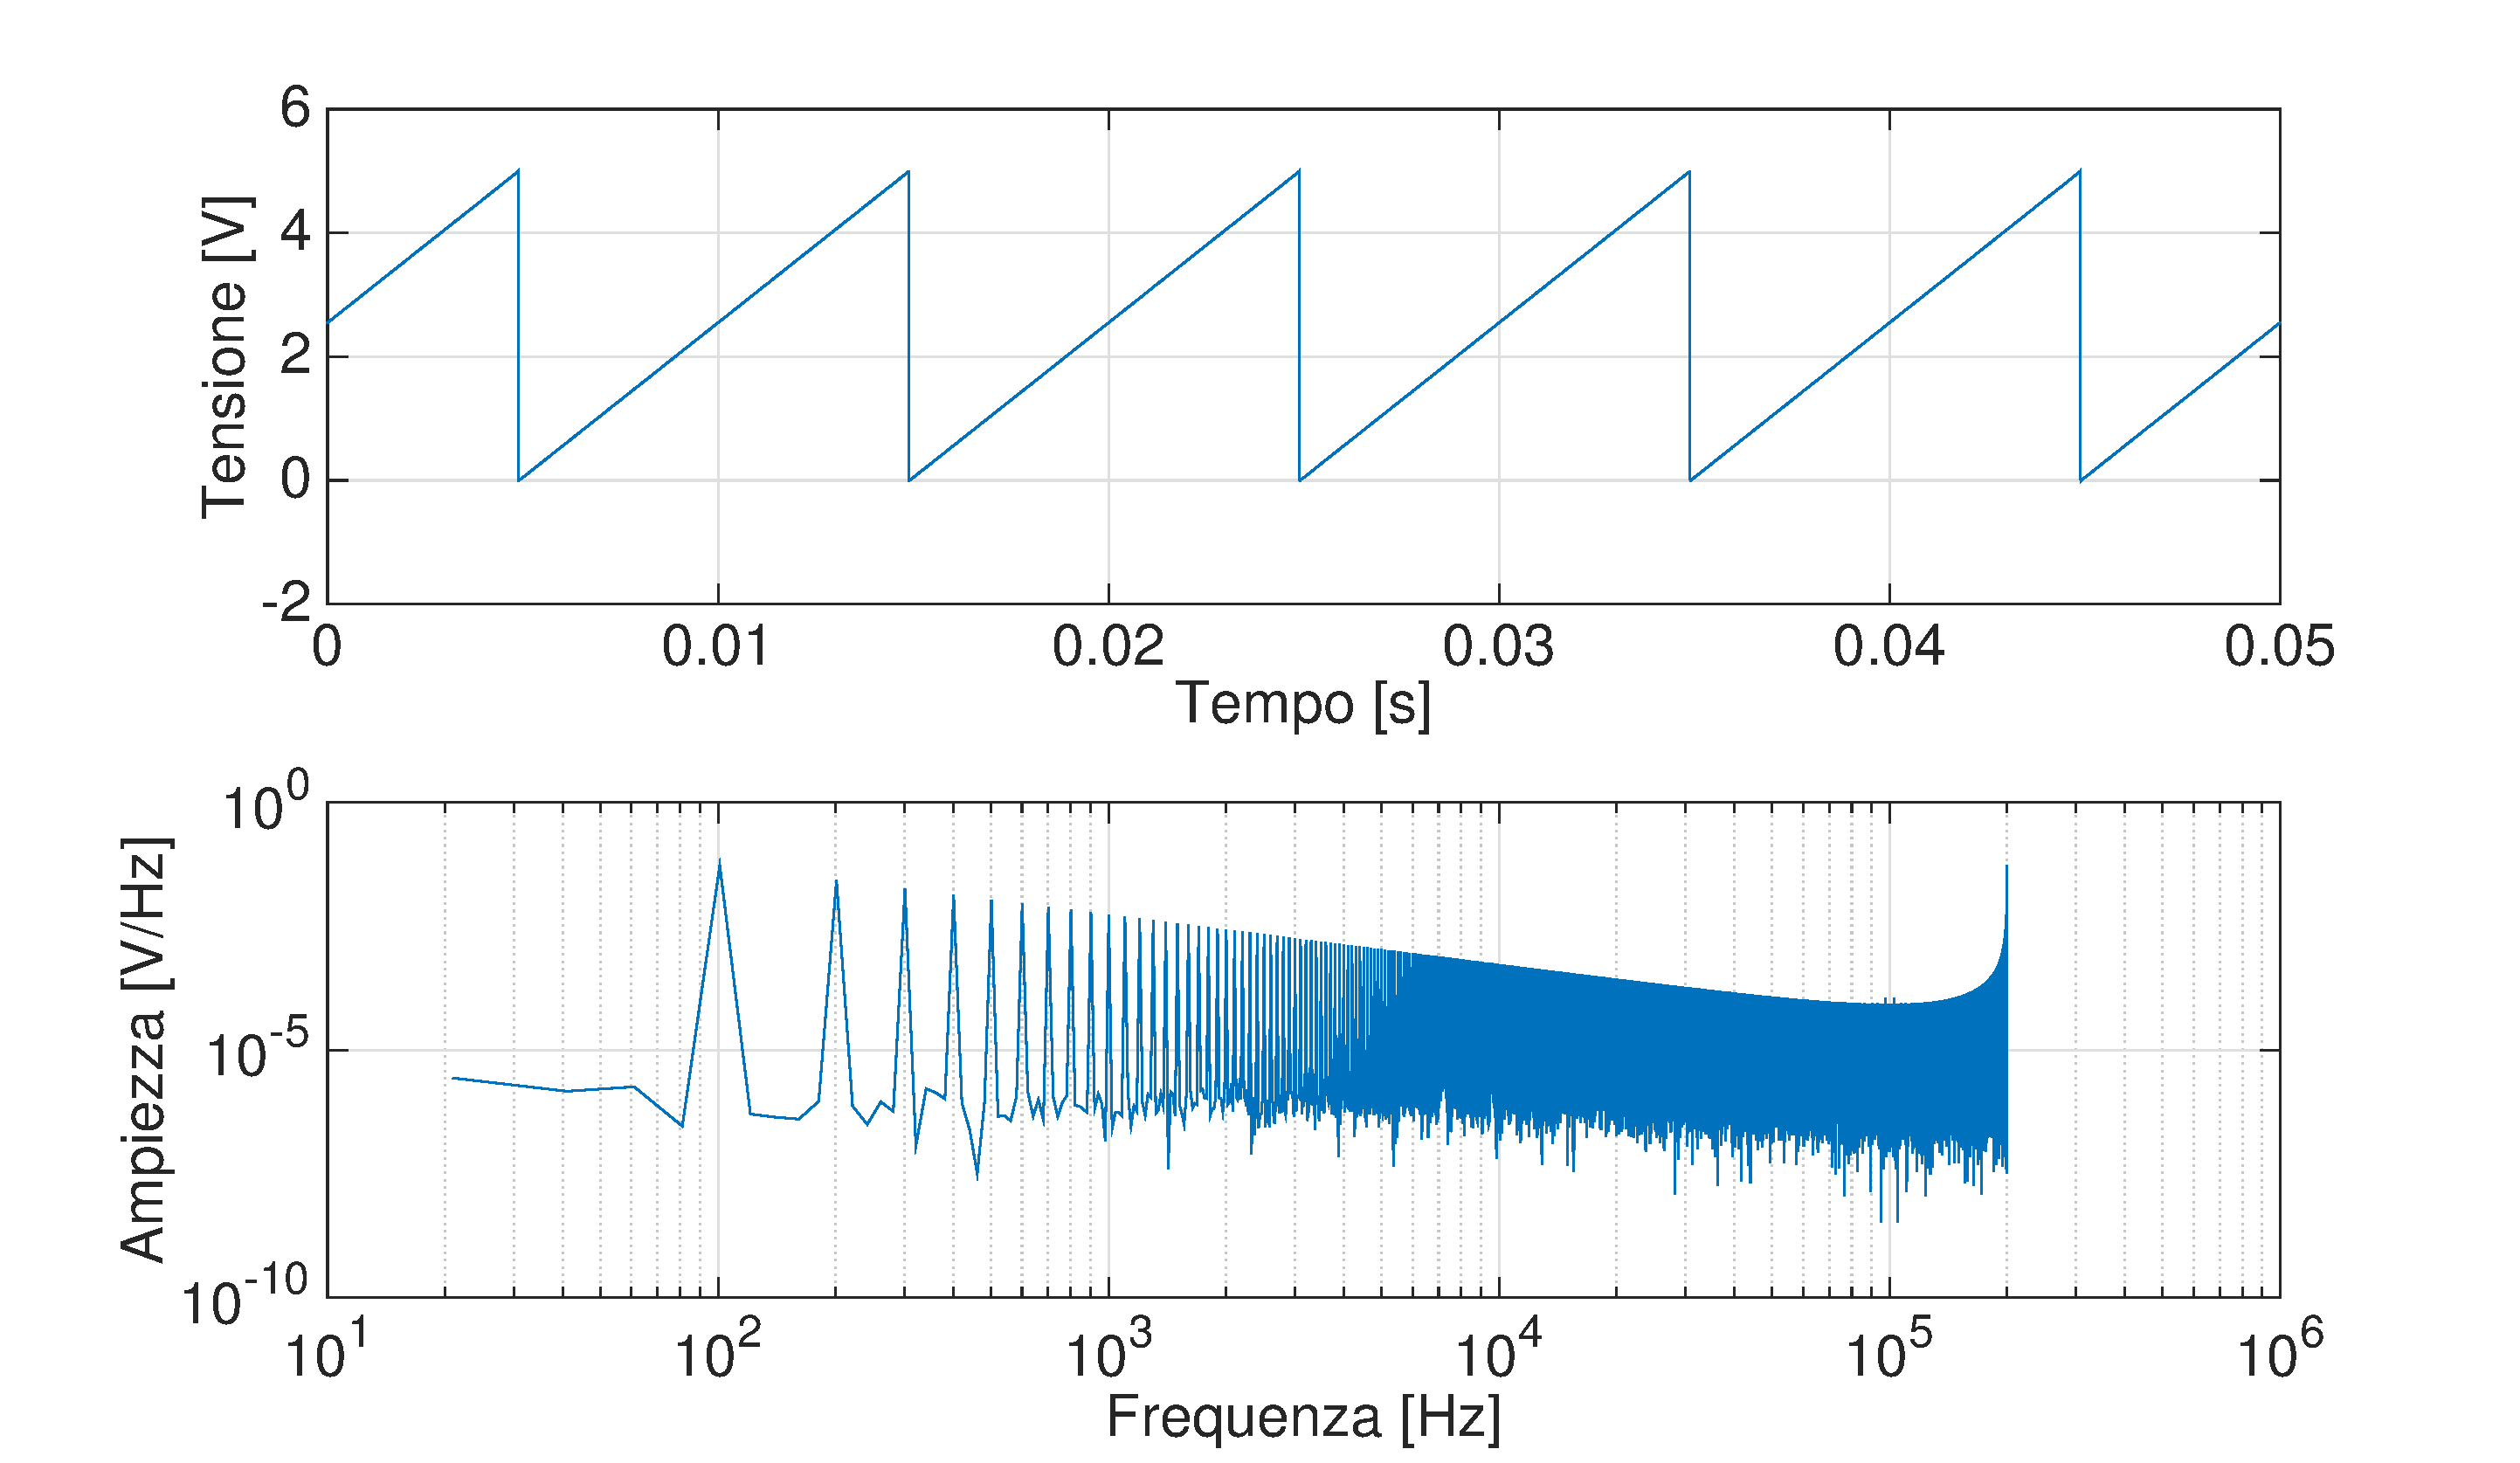
\includegraphics[width=.73\textwidth]{../E13/latex/sega100hz@10000,200000.pdf}
	\caption{Notiamo che abbiamo dei picchi sia sulle armoniche pari che dispari. Ciò è coerente con la teoria delle serie di Fourier sopra vista.}
	\label{sega}
\end{figure}

\subsubsection{onda AM}

In questa ultima parte abbiamo analizzato un segnale radio AM con $\nu_0=1\si{\kilo\hertz}$ e frequenza di campionamento $\nu_c=20\si{\kilo\hertz}$. Ovviamente il segnale è stato ricostruito senza distorsioni. Tuttavia in questo caso non è semplice calcolare la serie di Fourier sebbene sia possibile in quanto la funzione è periodica. 

\begin{figure}[H]
\centering
	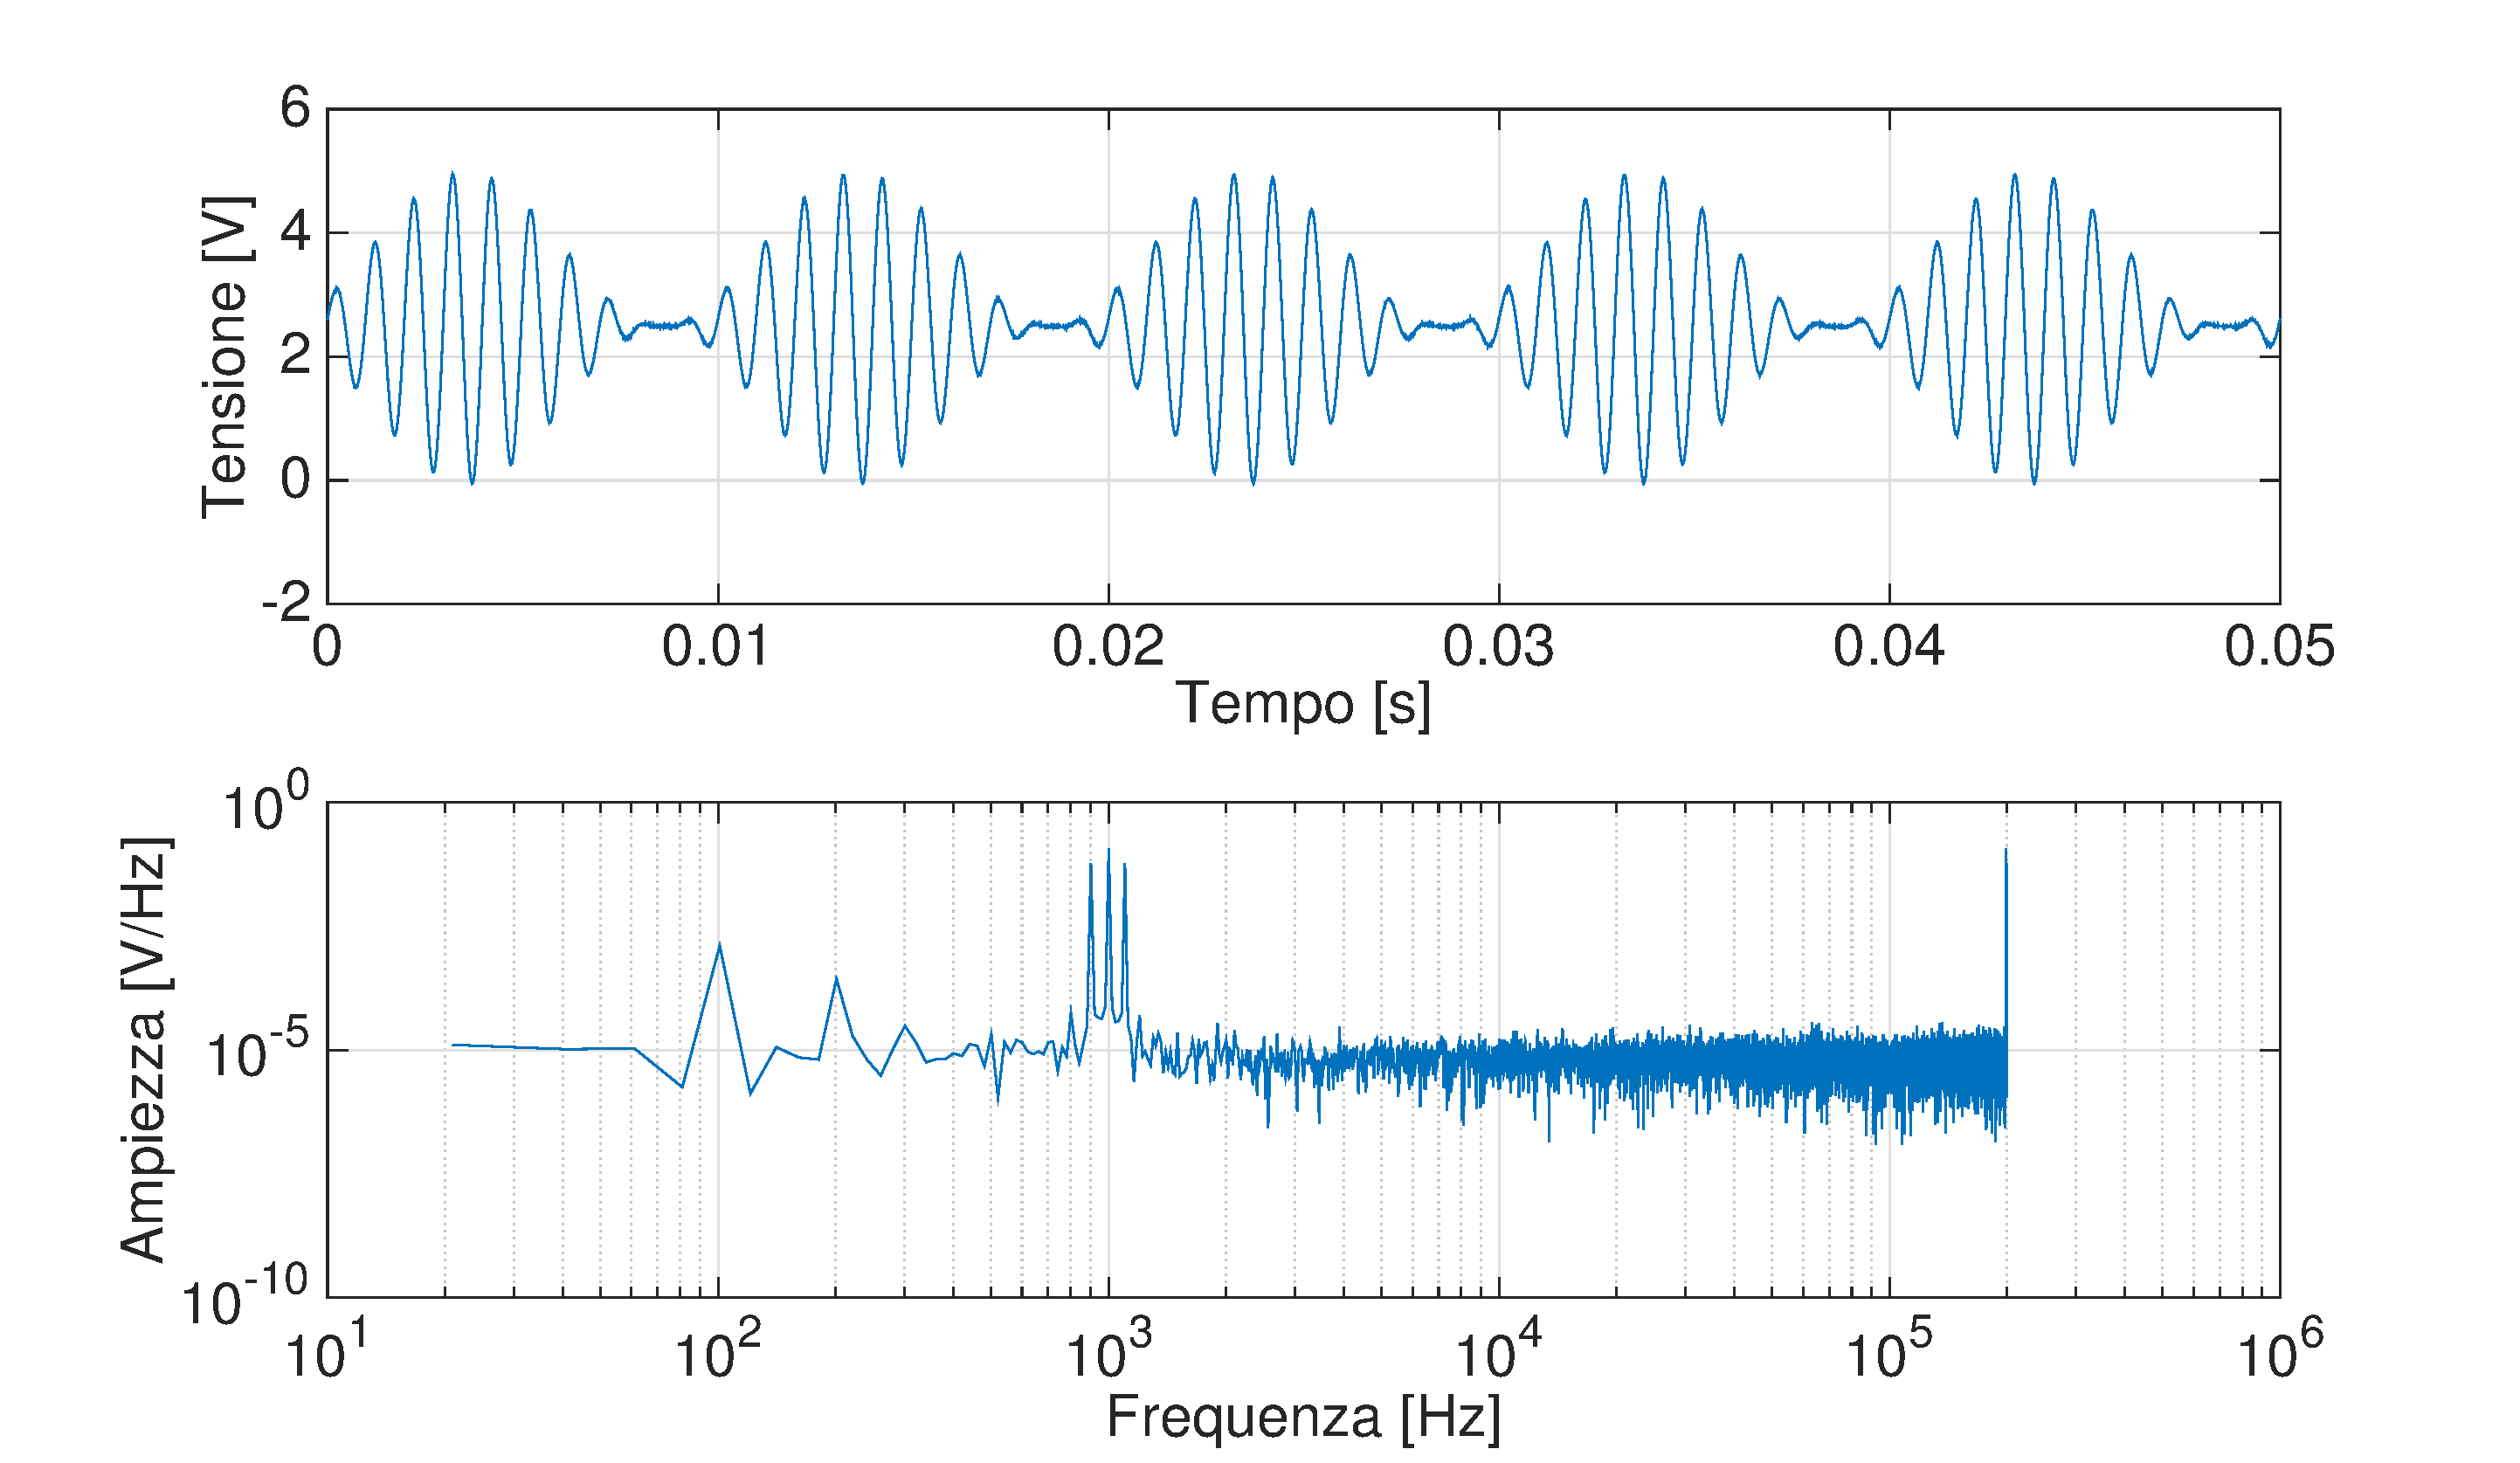
\includegraphics[width=.73\textwidth]{../E13/latex/am1000hz@10000,200000.pdf}
	\caption{Notiamo tre picchi di frequenza disposti simmetricamente rispetto a $1\si{\kilo\hertz}$.}
	\label{am}
\end{figure}

Osservando la FFT vediamo come vi sia la presenza di tre frequenze principali. Tali frequenze sono disposte a $1\si{\kilo\hertz}$, $\SI{900}{\hertz}$ e $\SI{1100}{\hertz}$. Quella centrale è detta portante mentre le altre due sono le bande laterali che ne modulano l'ampiezza.  Infatti, ricordando le formule di prostaferesi, possiamo vedere che il nostro segnale è del tipo $f(t)=Asin(\omega_1 t)cos(\omega_2 t)$ con $\omega_1 \approx 1 \si{\kilo\hertz}$ e $\omega_2 \approx 100 \si{\hertz}$. 

La presenza di diverse frequenze si traduce in una modulazione dell'ampiezza del segnale portante.



\subsection*{Conclusioni}

Abbiamo verificato il corretto funzionamento del convertitore analogico-digitale (ADC) e la validità del teorema del campionamento. Abbiamo inoltre verificato che in alcuni casi sebbene il teorema non sia valido in quanto non sono soddisfatte le ipotesi, è possibile ottenere comunque dei buoni campionamenti.
